
%% LLT: Turn off some annoying warnings...
\usepackage{breqn}
\RequirePackage{silence}
\WarningFilter{titlesec}{Non standard sectioning command}
\WarningFilter{scrreprt}{Usage of package}
\WarningFilter{scrreprt}{Activating an ugly workaround}
% **************************************************
% Document Class Definition
% **************************************************
\documentclass[%
	paper=A4,					
	twoside=false,				
	openright,					% doublepage cleaning ends up right side
	parskip=full,				% spacing value / method for paragraphs
	chapterprefix=true,			% prefix for chapter marks
	12pt,						% font size
	headings=normal,			% size of headings
	bibliography=totoc,			% include bib in toc
	listof=totoc,				% include listof entries in toc
	titlepage=on,				% own page for each title page
	captions=tableabove,		% display table captions above the float env
	draft=false,				% value for draft version
]{scrreprt}%

\newcommand{\thesisTitle}{Transients Notes}
\newcommand{\thesisName}{Carlos Arguelles, Aswathi Balagopal, Abhishek Desai, Sam Fahey, Raamis Hussain, Ali Kheirandish, Runze Li, Alex Pizzuto, Ibrahim Safa, Jessie Thwaites, Justin Vandenbroucke}
\newcommand{\thesisSubject}{Notes}
\newcommand{\thesisDate}{\today}
\newcommand{\thesisVersion}{Ongoing Draft}

\newcommand{\thesisUniversity}{\protect{University of Wisconsin - Madison}}
\newcommand{\thesisUniversityDepartment}{Department of Physics}
\newcommand{\thesisUniversityInstitute}{Wisconsin IceCube Particle Astrophysics Center}

\usepackage[utf8]{inputenc}		% defines file's character encoding
\usepackage[english]{babel} % babel system, adjust the language of the content
\usepackage[					% clean thesis style
	figuresep=colon,%
	sansserif=false,%
	hangfigurecaption=false,%
	hangsection=true,%
	hangsubsection=true,%
	colorize=full,%
	colortheme=bluemagenta,%
% LLT: Use biber if using UTF8 encoding
 	bibsys=bibtex,%
%	bibsys=biber,%
	bibfile=references,%
	bibstyle=alphabetic,%
]{cleanthesis}

\usepackage{amsmath}
\usepackage{amssymb}
\usepackage{tikz} 
\usetikzlibrary{shapes,arrows,positioning,automata,backgrounds,calc,er,patterns}
\usepackage{tikz-feynman}
\tikzfeynmanset{compat=1.0.0}

\hypersetup{					% setup the hyperref-package options
	pdftitle={\thesisTitle},	% 	- title (PDF meta)
	pdfsubject={\thesisSubject},% 	- subject (PDF meta)
	pdfauthor={\thesisName},	% 	- author (PDF meta)
	plainpages=false,			% 	-
	colorlinks=false,			% 	- colorize links?
	pdfborder={0 0 0},			% 	-
	breaklinks=true,			% 	- allow line break inside links
	bookmarksnumbered=true,		%
	bookmarksopen=true,			%
	colorlinks=true,
    linkcolor=black,
    filecolor=magenta,      
    urlcolor=cyan,
    citecolor=magenta
}

\usepackage{xcolor}
\usepackage{listings}
\lstset{basicstyle=\ttfamily,
  showstringspaces=false,
  commentstyle=\color{red},
  keywordstyle=\color{blue}
}


\begin{document}

\renewcaptionname{english}{\figurename}{Fig.}
\renewcaptionname{english}{\tablename}{Tab.}

\pagenumbering{roman}			% roman page numbing (invisible for empty page style)
\pagestyle{empty}				% no header or footers
% !TEX root = ../thesis-example.tex


% ------------------------------------  --> main title page
\begin{titlepage}
	\pdfbookmark[0]{Titlepage}{Titlepage}
	\tgherosfont
	\centering

	\vspace{3in}
	{\Huge \color{ctcolortitle}\textbf{\thesisTitle} \\[20mm]}
	
	\vspace{2in}
	
	{\large \thesisName} \\
	
	\vspace{3in}
	
	\textsf{ \thesisUniversity} \\
	\textsf{\thesisUniversityDepartment} \\
	\textsf{\thesisUniversityInstitute} \\
	\vspace{0.4in}
	
	\includegraphics[width=6cm]{images/WIPAC_logo.png} \\[2mm]
	\thesisDate \\

\end{titlepage}
		% INCLUDE: all titlepages

\setcounter{tocdepth}{2}		% define depth of toc
% \tableofcontents				% display table of contents

% --------------------------
% Body matter
% --------------------------
\pagenumbering{arabic}			% arabic page numbering
\setcounter{page}{1}			% set page counter
\pagestyle{maincontentstyle} 	% fancy header and footer

\chapter{March 19, 2019}

\section{ANITA Paper \& Regeneration}
\label{ANITA}
We had a ``brief'' discussion of the ANITA work (1 hour). We mainly discussed some subtleties that surfaced last Friday. 

\subsection*{\textbf{Instantaneous Data Quality}}
This depends on the final $N_{i3}$ that Ibrahim calculates, but we may be in a few different regimes for expected number of signal events. First, if the number of events would flood the detector on short timescales, we need to make sure that there are no detector failures (JEB failures). We might also be in the realm where the total integrated charge exceeds the EHE threshold, so we may want to make sure there are no EHE events. Third, events could not pass our analysis cuts, or finally, we might get lucky and get the perfect expected number of events at analysis level that wouldn't flood the detector. Ideally, we would look at lower level data to investigate this, but should not do that before asking WG leads. 

\subsection*{\textbf{Opening Angle}}
We have been neglecting the opening angle of the interactions along the trajectories. We can figure out if this is an important effect by doing a back of the envelope (there are methods that exist for approximating this with widening Gaussians). 

To do this rigorously, Ibrahim will need to save the intermediate energies along paths, and sample from opening angle distributions (or just take the RMS angle) and distribute it appropriately in 2 angular dimensions. The extent of the resulting cone will give us a penalty factor on the flux that is actually detectable. 

Sam notes that because we are looking at a flux from a point source, we might not need to do this, for every event scattering out of the line of sight, there will be another event that scatters into it, to first order. 

\subsection*{\textbf{Tracking Secondaries}}
We should also track $\nu_{\mu}$ and potentially $\mu$ fluxes that are the result of some of the interactions. 

\subsection*{\textbf{Debugging the Code}}
Ibrahim will continue looking into that bump that is evident when comparing his code to nuFATE for hard spectra. His plot agrees with Mary Hall Reno's paper. Carlos will look into the plotting scripts as well, as he is skeptical of Ibrahim's script. 

\subsection*{\textbf{Remaining Calculations}}
The main remaining calculation is effective area. Ibrahim and I will work on this. 

\subsection*{\textbf{Paper Planning}}
I will send an email to Dawn asking for the paper outline to be pushed back. This will give us time to work out with PubCom whether or not we want 2 papers as well as finalize some plots.  

\section{Gravitational Waves}
\label{GW}

\subsection{\textbf{Erik's Questions}}
First discussed questions from Erik:

\subsubsection{Q: What is the time for an upper limit or p value?}

Erik seems to advocate for upper limit as a function of declination, a la the other argument in the ANITA debate and some historic papers. 

Right now, calculating upper limits is $\mathcal{O}$(1hour). Raamis could work on speeding this up if we are willing to potentially sacrifice some accuracy.

I proposed looking into what Justin suggested a few weeks ago: calculating an average sensitivity by integrating sensitivity over the LIGO skymap.

\subsubsection{Q: What is the status of automation?}
Raamis seems ready with the automation. Some things are just being finalized on the realtime nodes. 

Justin asks for a sample GCN with filled in numbers in the case of a detection and non-detection. Raamis has these, but hasn't pushed to a website. 

\subsubsection{Q: Is signalness included?}
In the case of multiple neutrinos, you would rank it by the local TS. Justin suggests calculating the p-value as if the other events were not there. 

Some other things that came out here: the LLama people have been showing sensitivity as a function of declination of the injected source position. How will they quote an upper limit in the case of an actual detection when the true source position is not available?

\subsection{\textbf{Auto Tests}}
There are a few problems with interfacing with the realtime nodes, but Raamis is working on this. 

Default suggested by Justin: Launch jobs, p-value comes back in a few minutes from precomputation. If interesting, publish GCN automatically and immediately. If p=1, wait until UL is available, then publish GCN. 

\subsection{\textbf{Discovery Potential and Paper}}
Doga showed a discovery potential curve, Raamis can digitize this plot to do an overlay with his analysis. 

Strategically, LLAMA might get approval to unblind O2 on Thursday and might start working on a paper. Justin suggested taking a paper outline to Nu-sources on Monday, because we don't want to be in the position where the Columbia group begins a paper and then Raamis starts working on a paper after them even though O2 unblinding was earlier.  Raamis will email WG leads asking for a spot on the Monday call. Possible Proposed Title: \emph{IceCube search for neutrinos in coincidence with the first 11 detected Gravitational Wave Events}.

Raamis is also going to mention the timescale of the analysis in his email to remind people that GFU latency needs to be factored into analyses and that analysis time metrics should be compared to the time after the last relevant data packet is transmitted to the North. 

\section{Raamis' Paper Outline}
\begin{my_list_item}
    \item Maybe add that you are open to changing journals
    \item Add time window to the abstract, get rid of time
    \item If you are going to describe the Prior, Josh recommended taking a look at Rene's 8 year paper
    \item Mention that the circles around events are certain percentage (90) uncertainty
    \item Include an example TS distribution (Justin also suggests including the passing fraction plot)
    \item Label colorbar. Justin suggests just including the colorbar in the corner of the overall figure, maybe do the same for Equatorial and GFU event
    \item You could include a slide discussing just using the typical IceCube point source sensitivity but only in the region of the LIGO PDF
    \item We also discussed doing a similar type of precomputation for signal injection but just for point sources for a bunch of declinations across the sky, not using the Prior Injector. 
    \item Moving on to analysis specific stuff: Would you be able to update the sensitivity with Doga's new sensitivity?
    \item If you send this in an email to Erik, would you be able to ask for the skymaps again in that same email?
    \item It might be worth discussing with Erik and Benedikt about getting a dedicated followup server
    \item You might want to add some bullet points to the latency slide: add some metrics and some details, mentioning filesystem crashes, both analyses have to wait 500s. Josh thinks you might want to show it on Monday, Justin might want to hold cards close to the chest and not show it yet. 
    \item Something to think about is maybe building likelihoods before the end of the time window
    \item Would you be able to check how many CPUs are on the realtime nodes?
    \item GCN comments: 90 percent PSF is awkward phrasing, if greater than 3 sigma, just say that
\end{my_list_item}

\chapter{March 26, 2019}

\section{FRB Paper}
Sam is in Minnesota and Ali is still out of town. Sam is forwarding me the list of comments, and we will discuss who can respond to what comments. 

\section{ANITA}
Ibrahim and I have been asking around about muongun simulation. First, we were directed to HESE simulation, but all the muongun was downgoing (no simulation below the horizon). The lead we are currently investigating is from a diffuse analysis done in 2012. There is muongun simulation processed to l1, l2, and l3. It is poorly documented, so I am looking at the files to try to determine the underlying simulation distributions, and Ibrahim is figuring out if simulation from 2012 (ie before pass2) will work with Tessa's event selection scripts. 

\section{Gravitational Waves}
Raamis is working with Erik on GCN templates, examples in his Wiki. As for reporting upper limits, Raamis has been working on calculating the standard point source sensitivity (no prior) for 5degree bins in declination across the sky, and then the best and worst for within the 90\% containment could be cited.

We also spoke a lot about the conversation on fitting for underfluctuations, specifically in limit setting. Ibrahim advocates for using underflucuations for more constraining upper limits. On the call it was mentioned that Raamis might be able to show that he could also set more constraining limits if he were to fit for underfluctuations, but I raised a potential problem with this (there is essentially no way to get a negative TS value based on the way that the spatial prior analysis works, because the pixel with the highest LIGO weight is not penalized at all, so that pixel is guaranteed to have a TS$\geq 0$).

Raamis sent an email to Scott asking for GCN circular submission credentials, and I am helping with writing a script to call people to wake us up if a LIGO alert comes overnight. 

\section{Collaboration Meeting Planning}
Briefly discussed planning for the collaboration meeting. Raamis is hopeful that there will be some new LIGO events to discuss during a Nu-Sources or Realtime parallel, and I am hoping to finish the grbllh/Skylab Fast Response conversion and present that in Realtime. We are also open to more talks if anyone has suggestions. 



\chapter{Phonecall with FRB Paper Reviewers, March 29, 2019}

Kevin didn't show up. As we waited, Segev asked what comments are going to be hard to address. Ali said that a lot of the comments from Kevin are stylistic. Brevity was intended, because there are a lot of previous papers.

Lutz said that the comments in the Supernova section are good and should be followed. He also does not like using the Lawrence-Livermore model, and thinks that the limits should be presented in a more general context. Erin agrees with that. Lutz says that you could leave the limit in terms of some $\alpha$ parameter, but Justin likes having a quantitative limit. Lutz says that this can still be done if you assume certain widths and energies, but then readers can reinterpret for different widths and energies. 

Juanan advocates for settling these issues before going to collaboration review. Other comments from Juanan:

\begin{itemize}
    \item Confusion around the different numbers of FRBs
    \item Requests a sentence maybe about the repeater
\end{itemize}

Ali said that he and Sam could probably post a new version on Monday. Reviewers will aim to give feedback by the end of next week. Erin recognizes changes the SNDAQ limit might take some more time, Juanan is fine if that work is still ongoing as the paper goes into Collaboration review. 
\chapter{April 25, 2019}

\section{Plenary Talk Reviews}
\subsection{ANITA}
Ibrahim and I gave a practice ANITA plenary talk. We decided to not discuss the SNDAQ information, and to move the dead time discussion into the Followup sections, in addition to adding a plot with upper limits. A more comprehensive conclusion slides needs to be made, with mention of the application of TauRunner to other high energy problems.

\subsection{Gravitational Waves}
Justin and I think Raamis should emphasize that you perform a lot of background trials for the specific skymaps (emphasizing the statistics that you can gather with such a short latency).

Justin suggested asking for the realtime results from the Columbia group.

Justin's suggestion for a title tweak: \textit{Results from the archival and O3 Realtime Neutrino Follow up of Gravitational Waves}. He also suggests adding contours to GW localizations for the talk, not necessarily in realtime though because the marching triangles algorithm takes time.

I mentioned that another disadvantage of using the simulated skymaps for the Columbia analysis is that if there is any data/MC disagreement for skymaps on the LIGO end, that this will propagate into the Columbia analysis, but not Raamis's analysis. 

\section{ANITA regeneration paper}
Ibrahim also showed the paper outline for the regeneration paper. Francis had suggestions to declutter the plot comparing different injected neutrino energies with their secondary distributions to the analytical suppression. Carlos wants a vertical line at the injection energies, not bins, and then binning the smaller energies. I suggested moving the y limits lower to see the highest energy bin for the highest injected energy.

Justin asked for an increase in statistics in the exit probability jobs.

We also discussed the Eddington bias when comparing to the HESE flux. For that reason, we decided to use the HESE flux to set the maximum allowed flux that ANITA could have seen, not using the best fit of ANITA to look at how much it overshoots the HESE flux.

We decided to send an outline to PubCom today so that we can start working on the paper because we are worried that it could get scooped. 

\chapter{Madison Collaboration Meeting, Neutrino Sources}

\section{Parallel Session Number One}
\begin{itemize}
    \item \textbf{Overview on Tools and Analyses (Josh)}: Gave an overview of all of the tools we can use to do point source analyses. Began a discussion on trials correction for all of the different analyses
    \item \textbf{Path towards new PS Likelihood (Theo, Hans, and Martin)}: Starting from first principles, rederives PS likelihood. They extract PDFs from Monte Carlo using KDE techniques, trying to be smart about the high dimensionality. They argue that per event their rigorous treatment reduces to only two spline evaluations. Nice feature is that the KDE seems able to localize sources. 
    \item \textbf{Determining Time Dependence (Ignacio, on behalf of Pranav)}: Taking an already found signal in time-integrated data and determining if there is underlying temporal behavior. The TS is essentially the magnitude of the difference between the CDF of the coincident events as a function of time vs a constant rise hypothesis (steady-source hypothesis). Shows comparison to the ideal cases (injected at a delta function at the very beginning or very end of the livetime). \emph{Question}: there are some background events that contribute, and their behavior isn't truly time independent. Would this be possible to include? Ignacio says that this wouldn't be hard to implement.
    \item \textbf{Periodic Neutrino Sources (Chun Fai Tung)}: X-Ray and Gamma-ray binaries are expected to be periodic sources. 4 proposed searches: triggered with fixed period, catalog with unknown period, time-integrated catalog search, and a population analysis. He shows how well his method can recover flares with different underlying periodicities, but is worried about computational costs.
    \item \textbf{Search for Binaries (Qinrui)}: Investigating microquasars (binaries with jets) and some other binary systems. Difference between this and Chun Fai's analysis is that this analyses uses lightcurves from Swift-BAT (and then apply Bayesian Blocks to identify flares) to build the time PDFs. Sourcelist from WATCHDOG (BH X-ray binary list from the last 20 years). Qinrui shows some sensitivities and discovery potentials for a few examples of light curves. Qinrui is currently investigating the best way to include sources of interest that are not included in WATCHDOG.
\end{itemize}

\section{Parallel Session Number Two}
\begin{itemize}
    \item \textbf{Tidal Disruption Events (Robert)}: Robert showed an overview of his TDE analysis as he is working towards a paper outline. Analysis method fits source weights individually, in case TDEs are not standard candles. Unblinded p-values are consistent with background. Some TDEs were analyzed individually, again, consistent with background. Limit calculation assumes a weighting scheme. Robert discusses prospects for sensitivities and rate estimation with new detections of TDEs, especially from ZTF, and so he hopes to update the analysis in the future. \emph{Questions}: Markus asked how you can set such constraining limits (below the diffuse flux) with only a few TDEs. I asked about how much the assumption of stadard candles changes the limits.
    \item \textbf{Extended Source Analysis Update (Devyn)}: Many extended sources with few-degree extensions detected by HESS and HAWC in high energies. For source extensions as small as 2 degrees, sensitivity is order of magnitude better than PS likelihood when extension is taken into account. Devyn shows that she does not reproduce a bug(?) from the historic analysis when she is rerunning it. Devyn is puzzled by the fact that signal subtracted likelihood is pushing the background distribution in the wrong direction. With different background parameterization, the behavior is as expected, but there is some odd behavior now when comparing the KDE and Splined BG TS distributions. Devyn also summarizes Mehr's work in Skylab with Tessa's sample. Some questions were raised about odd structures in zenith PDFs. 
    \item \textbf{Untriggered, time-dependent blazar search (Erin)}: Erin presents an unblinding request for the untriggered flare analysis on the Fermi 3LAC catalog using the diffuse sample. Significance will be calculated using a binomial test of the population (with correction for correlations between blazars). Erin mainly focused the presentation on the decorrelation method that she is suggesting because the rest of the analysis is using standard methods. \emph{Questions}: Greg asked if you need to be so severe as to remove an entire blazar when decorrelating instead of just assigning events to single blazars and not both.
    \item \textbf{GRB Precursor and Afterglows (Kunal)}: Kunal mentions that historic GRB analyses only considered the prompt phase of GRBs, and he is interested in extending to the precursor ($\mathcal{O}$(weeks)) and the afterglow ($\mathcal{O}$(months)). He chooses the data to inform him how long of a time window he can afford to look at for the precursor and afterglow. He shows a discovery potential curve as a function of the time window. I'm concerned that he is extrapolating his TS distribution according to a $\chi ^2$ that doesn't fit well, may just want to use a 3$\sigma$ discovery potential. \emph{Questions} What is the confidence level for the discovery potential? 50 percent. Markus brought up that the two discovery potential curves on slide 7 should be identical if just a simple box is used, but Kunal explains that the time window is fit for, $T_0$ just reflects the injected signal timescale. Ignacio is concerned that the proper likelihood is not being used, and suggests iterating offline. 
    \item \textbf{GRB Precursors (Paul)}: Paul wants to used identified precursors, which makes his analysis separate from Kunal's which fits for emission timescales for all GRBs. Paul wants to use the standard transient likelihood, but just with larger time windows to include the precursor stage, using GFU and a list of GRBs from GRBweb with identified precursors. For GRBweb, all Paul needs to do is move the SQL database from his local machine to the Madison servers. Paul has a way to obtain healpix maps of GRBs detected by Fermi-GBM, and he compares to the mismatch that was obtained when treating the burst uncertainties as 2D-gaussians. Paul then discusses identifying precursors, which he has to do himself. He is using a Bayesian Blocks approach on the public Fermi-GBM data, and is trying to reproduce old Fermi-GBM results. \emph{Questions}: Are you analyzing just the precursor time window or doing the analysis from the beginning of the precursor until the beginning of the prompt phase. This study will be done.
    \item \textbf{GRB Coincidence Analysis (Liz)}: Liz presents an update on a per GRB analysis from 2011-present with the hopes of eventually scaling to a realtime analysis. Liz is suggesting using the GRB $T_{100}$ and then adding extra time to the time window in an expanding time window method. She shows the sensitivity of the analyses for different time windows and different temporal patterns for signal injection for a test case at a declination of $\delta=+11.5^{\circ}$ with a $T_{100}=$24.6 s. Liz calculates the effective trials factor for correlated expanding time windows. She suggests comparing the p-value from the $T_{100}$ window and comparing it to the best of the rest of the expanding time windows.
\end{itemize}

\section{Parallel Session Number Three}
\begin{itemize}
    \item \textbf{ESTES Event Selection (Manuel on behalf of Sarah)}: ``Saruel'' presents a technical overview of the ESTES event selection. ESTES defines an event specific dark region to declare the veto, which increases the effective volume. Veto is determined by starting at the first lit DOM, looking at photon tables, and calculating a probability that a muon could have snuck by to that DOM without making any previous deposits. \emph{Questions}: Ignacio asked if there is an effective minimum number of outer layers that function as a veto. Manuel says no, as few as one is fine.
    \item \textbf{Neutrino Source Cascade Dataset (Steve)}: Steve shows progress he has made on a cascade nu-sources event selection. Improvement in southern sky because cascades do not require a large energy threshold to cut out background. Historic MESE sample relies on hardcuts, goal is to not require hardcuts and veto to improve effective volume, and use the DNN reconstruction for the events. Angular resolution from DNN trained on cscdl3. Method currently performs better than MESC at low energies, worse at higher energies. Improvement in sensitivities for softer spectra, no gains in hard spectra because of this behavior. \emph{Questions}: Do you think the estimated errors are good? Steve has not yet checked Data/MC agreement nor how accurately the Gaussian approximation works.
    \item \textbf{Multiflare Stacking (Will)}: Will began with a refresher of his multiflare analysis. Will is using a binomial approach to stacking flares, which is essentially a multiflare extension of Erin's single-flare binomial stacking. Will has begun working on multiflare skymaps, i.e., not using a source list and just performing his analysis on the entire sky. This is a ``Computational Nightmare,'' so Will is debating moving the analysis to cSky to accomplish this part of the analysis. Will also points out that multiflare stacking is complementary, not meant to replace, single flare analyses.
    \item \textbf{ZTF-IceCube Analyses (Anna on behalf of Ludwig)}: Of the last 7 IceCube alerts, only 1 could be observed (a doublet at the declination $\delta = +13^{\circ}$). Estimates for Gold events coverage is about 10 per year. Analysis considers the whole GFU stream as well as all current transients from ZTF. If deemed interesting, you can trigger spectroscopy follow up in ZTF. Filters transients brighter than 19th mag, complete up to 18.5 mag. Anna describes the logic behind triggering observations.
    \item \textbf{Self-triggered PS analysis (Martina)}: Martina proposes using the TXS analysis on all alert events, i.e. using the HESE tracks and EHE events as a ``source catalog.'' Sky is divided up into Cartesian grid positions with a width of $0.1$ degrees. Martina suggests at each source doing a time-integrated search and a time dependent (single flare) search. She suggests doing both a stacked and max-burst analysis for the continuous emission, and for the flare followup only doing a max-burst search. \emph{Questions:} Questions were brought up about trials factor and how Martina is taking into account the uncertainty information on the alert events. Qinrui asked about whether or not the signalness is taken into account. Justin asked if there is overlap with the fast response analyses. What Martina calls the ``transient'' analysis is the untriggered flare fit. I wonder why she doesn't take the full likelihood information into account, which we have for the events.
    \item \textbf{UHECR Analysis (Lisa)}: Lisa presents an unblinding request for her UHECR analysis. This is mainly an extension to the analysis that was unblinded before Stockholm, namely, with larger datasets. Lisa is also rerunning some signal injection(?) in a slightly different manner, but beyond that, the analysis is very similar and meant as a complement to Anastasia's analysis.
\end{itemize}

\section{Gong Talks}
\begin{itemize}
    \item \textbf{Mixed proton-iron composition in UHECR analysis (Lisa)}: Lisa presented an update on Phillip's work on how a different assumption on the cosmic ray compisition would affect the UHECR-nu correlation analyses (specifically with the size of the uncertainty regions because different elements have different rigidities)
    \item \textbf{Novae with GRECO (me)}: I showed some signal and background estimates for novae assuming negligible gamma-ray absorption
    \item \textbf{Upper limit calculation for GW-nu analyses (Doga)}: Doga discussed how to appropriately set limits in a way that does not take into account irrelevant information
    \item \textbf{Neutrinos from AGN cores (Robert on behalf of Federica)}: Says that accretion disks are prime candidates for neutrino production, assuming neutrino production is proportional to luminosity of AGN cores. There are a lot of sources, Federica is looking into how to deal with this.
    \item \textbf{SkyLLH (Martin)}: SkyLLH sales pitch.
    \item \textbf{Counting experiment sensitivity in different background regimes (Me)}: I talked about a weird dip feature that shows up in low background analyses when integrating over a small but non-negligible amount of background
    \item \textbf{Kinematic angle (Paul)}: Paul actually does the full calculation for the kinematic opening angle for charged current interactions. He especially notes the long tails of these distributions that are often neglected.
    \item \textbf{Datasets update (Liz)}: To unblind, the data curator now needs to approve the dataset. Approved datasets have the advantage of not needing to go through this procedure. Liz suggests buffering unblinding by about a week to account for this process if you are not using an approved dataset
    \item \textbf{Optimizing optical followups (Robert)}: Robert suggests being proactive, ie, defining if you want a pure, large, biased, or nearby sample. To do this, you should simulate the source population before just going after one.
    \item \textbf{Realtime alerts from HESE Cascades (Hugo)}: It can be helpful to include HESE cascades for short timescale transients. Hugo presents some preliminary work towards this.
    \item \textbf{HESE Skymap scans (Robert)}: The HESE team needs sky scans of the HESE events (overall about 30 scans need to be done), and Robert is working on them. These scans are slightly different from the realtime scans, and Robert notes the differences between them.
    \item \textbf{Hydrangea Followup (Sarah)}: Sarah wants to followup Hydrangea using the same methods as the transient search for ANITA. \emph{Questions}: Why no time-integrated search?
    \item \textbf{Exploring counterparts of high energy neutrino events (Lisa on behalf of Pratush)}: Lisa discusses a proposed cross-correlation analyses between the Swift-BAT catalog and IceCube data 
    \item \textbf{X-ray and UV/O search from joint GW-nu coincidences (Azadeh)}: Azadeh discusses Swift Follow-up observations of joint GW-nu coincidences. Azadeh was appointed 4 priority 1 approved triggers, and will trigger on coincidences with FAR of no more than 2 yr$^{-1}$.
    \item \textbf{Spline MPE/Paraboloid (Jimmy)}: Jimmy airs our dirty laundry behind Spline MPE and Paraboloid likelihood spaces. He especially notes that Wilk's breaks down at high energies from an increase in stochastic losses. Minimizer fails to find the global minimum around 10$\%$ of the time
    \item \textbf{Blazar stacking limits (Matthias)}: Matthias unblinded the analysis correlating with the 3FHL catalog. Limits are at the 10-20$\%$ level of the diffuse flux for different assumed spectra. He proposes an update that would use 4FGL and more IceCube data, and additionally fitting for the distribution of blazar spectral indeces.
    \item \textbf{DECam search for optical transients (Rob and Keith)}: Rob discusses his analysis searching for explosive optical transients in coincidence with TeV-PeV neutrinos. DECam gets down to about 23-24 mag, so they can probe really deep sources, specifically looking for core-collapse supernovae. Rob shows that signal and background is separable on a statistical basis
    \item \textbf{Astrophysical neutrino catalog (Ignacio on behalf of Charles)}: The idea is to have a website with all of the information about published, likely astrophysical, neutrinos.
    \item{ \textbf{Next Steps in FRB Analyses (Justin)}}: Justin talked about FRB detection rates as well as prospects for future sensitivities with a larger source class.
\end{itemize}
\chapter{May 9, 2019: Meeting Minutes}

\cleanchapterquote{We can have a paper outline ready to go to the analysis call two weeks from today}{Ibrahim Safa}

\section{ANITA Papers}
We discussed the plot we want from the regeneration work to go into the collaboration paper. Namely, use the upper limit from the point source results over the central 90\% energy range of the point source analysis, and then fit for the ANITA flux to calculate an upper limit and compare to the implied ANITA flux (similar to the HESE plot, but now without the solid angle dependence).

\section{Gravitational Waves}
Raamis found and fixed a bug in quoting a range of upper limits in his analysis. The bug came from a treatment of quoting the range that didn't account for discontinuous priors. Only one GCN circular was affected. 

\cleanchapterquote{This is definitely right now (I'm at least $3 \sigma$ sure)}{Raamis Hussain}

\vspace{0.01in}

There was a lot of discussion on negative TS values during the collaboration meeting. One method for fixing it:

\begin{equation}
    \frac{d(TS)}{dn_s} = 2 \left[ -1 + \sum_{i=1}^N\frac{S_i}{n_sS_i + n_bB_i} \right]
\end{equation}

This leads to some \textit{weird} TS distributions. I asked for what this looks like in terms of number of events. Justin suggests doing a sort of coverage test. In other words, actually inject a physical flux and then see which method recovers the injected flux a higher percentage of the time. 

Using this method, there are 3 different populations for TS values. A peak at $-\infty$ when there are no events on the sky, highly negative values for events nowhere near the contour, and those with events near the contour. At the collaboration meeting, it was decided to write a joint paper with the Columbia folks. Raamis has fixed the rotation for the maps. 

Imre mentioned in the paper potentially also following up the known galaxy location of the BNS and not just the LIGO skymap. 

Justin also had a few suggestions for internal reports: 

\begin{enumerate}
    \itemsep-0.75em 
    \item Accounting for multiple updates (Preliminary, initial, etc.). Raamis has implemented this
    \item Mention that times are UTC (truncate to nearest second)
    \item Sometimes the date interval on the x-axis is unclear
    \item The two skymaps are inconsistent in units (one in degrees, the other in hours)
    \item Per event p-values are only using the best fit location, but I argued that this isn't what the analysis produces in terms of a p-value. It is computationally expensive to evaluate the p-values using only certain events on the sky.
\end{enumerate}
\chapter{GRBLLH Fast Response Walkthrough}

Hey all, I'm headed out of town for 5 days (and will likely be without internet), so I wanted to write a brief how to in case there is an IceCube alert event and we need the fast response analysis. 

First, we want \texttt{py2-v3}:
\begin{lstlisting}[language=bash]
eval `/cvmfs/icecube.opensciencegrid.org/py2-v3/setup.sh`
\end{lstlisting}

Next, you want to initialize a specific \texttt{icetray} and go to the virtual environment I set up for just this purpose: 

\begin{lstlisting}[language=bash]
/data/user/apizzuto/software/icerec_V05_02/build/env-shell.sh 
source /home/apizzuto/.venvs/fast_response/bin/activate
\end{lstlisting}

Next, go to my directory where I have the fast response scripts (these also exist in the \texttt{icerec} environment, but I run the ones in my \texttt{/data/user/} because it's a copied version of a stable release and the one in my \texttt{icerec} is analogous to the trunk: 

\begin{lstlisting}[language=bash]
cd /data/user/apizzuto/fast_response_code/
\end{lstlisting}

I changed permissions just now so that everyone has read/write permissions in this directory. I'll change it back when I get back. Next, run the actual analysis. This is the code I used to run the analysis for the last IceCube event followup. 

\begin{lstlisting}[language=bash]
python run.py --ra=65.7866 --dec=-37.4431 --sigma=1.2 
--skip-events=132518:766165 --start="2019-05-03 18:26:49" 
--stop="2019-05-05 18:26:49" --name="IceCube 190504A Two Day"
\end{lstlisting}

\texttt{ra} and \texttt{dec} are the coordinates in degrees, \texttt{sigma} is the source extension in degrees (for IceCube events, the 90\% containment assuming the contour is radially symmetric). \texttt{skip-events} is the runID and eventID of the HESE or EHE event, just in case it ended up in the GFU sample. This can be found in the \texttt{Bacodine} email that gets sent to icecube-c, or by finding the event in \href{https://live.icecube.wisc.edu/auth/?next=/realtime/}{IceCube live}. 

This will calculate $TS$ and $n_s$ for the analysis and will create a subdirectory with the analysisID. If $p=1.0$, then you can calculate the upper limits right away: 

\begin{lstlisting}[language=bash]
python upper-limit.py $ANALYSISID
\end{lstlisting}

where \texttt{\$ANALYSISID} is the name of the subdirectory that was created. You can pass \texttt{trials=1000000} if you only want 1e6 trials, otherwise, it does 1e7. If you have a p value that is not 1, then you must first run the background trials: 

\begin{lstlisting}[language=bash]
python bg-trials.py $ANALYSISID
\end{lstlisting}

and then after this you would run the upper limit script. Once you have an upper limit, create the report:

\begin{lstlisting}[language=bash]
python report.py $ANALYSISID
\end{lstlisting}

Now, in the analysis subdirectory, there will be a \texttt{\$ANALYSISID\_report.pdf}, and this should be the final report. I tend to copy this into my \texttt{public-html}, but you could also just \texttt{scp} it. Then you should be done. Feel free to edit the wiki and upload to the Google Drive, or ask me and I can do it when I get back. Templates for GCN circulars are linked on the wiki, or can be found directly \href{https://wiki.icecube.wisc.edu/index.php/Fast_Response_ATel_and_GCN_Templates}{here}.
\chapter{May 16, 2019}

\section{ICRC Planning}
Timeline:
\begin{itemize}
    \itemsep-0.85em 
    \item Soft deadline for first drafts to be uploaded to Google Drive / overleaf: June 4.
    \item Final deadline for new analyses approved for unblinding: June 6.
    \item Hard deadline for first drafts to be uploaded to Google Drive / overleaf: June 11
    \item Final deadline for new plots to be shown in the analysis call: June 13.
    \item Final drafts of proceedings for collaboration review: June 25 (3 weeks before ICRC deadline)
    \item Final ICRC deadline for uploading papers is July 16.
\end{itemize}

June 4 is 2.5 weeks away, to iterate locally, try to send drafts beforehand (two weeks from today).

Unclear of what ``final deadline for new plots to be shown'' means, Raamis is following up with Ignacio or Segev


\subsection{Gravitational Waves (Raamis)}
For upper limits, Raamis might try to get on the next Neutrino sources call to discuss the new way to calculate upper limits, so that he might be able to put the new upper limits in the ICRC proceedings. 
\begin{itemize}
    \itemsep-0.85em 
    \item Unblinded skymaps with neutrinos and 90\% contours (archival and realtime)
    \item Background TS distributions, or possibly fit vs. injected flux
    \item (Updated) upper limits
    \item Table with all of the results
    \item Science / citation heavy introduction
\end{itemize}

\subsection{ANITA: Collaboration (Alex)}
ICRC proceeding that will be pretty much a copy of the journal paper. Possibly keep interpretation section short. I'll try to discuss with Anastasia next week. Could potentially get more into the likelihood analyses if it's easy. 

\subsection{ANITA: Few Author (Ibrahim)}
Hopefully we will have the few author paper out, and then we could essentially just promote that paper in the ICRC writeup. 

\subsection{FRB (Alex)}
Highlight the journal paper with representative plots from the L2 analysis and Ali's analysis. Include text about the prospects for future analyses. Could discuss realtime and reference fast response 

\subsection{Fast Response (Justin)}
Justin can lead paper writing. Plots / things that we need:
\begin{itemize}
    \itemsep-0.85em 
    \item p-value distribution
    \item Tables with all of the results
    \item Zoomed in skymaps of certain analyses
    \item False alarm rate plot
    \item Average latency or computing time
    \item Some performance plots
    \item Outlook for scanning source localization uncertainties
\end{itemize}

\subsection{DECO (Alex)}
Blake is happy to help with the writing, and Justin is back June 16th. I will aim to have a draft with Blake by the time Justin gets back. I will see if I can get Blake on the author list
\begin{itemize}
    \itemsep-0.85em 
    \item About a third general description and updating the world map (Blake?) Maybe avoid total user count in favor of world map
    \item About a third on CNN stuff, citing the paper
    \item About a third on new stuff (simulation and experimental). For the experimental stuff, let's try to get them classified and then compare the distributions. Probably avoid efficiencies in favor of classifications (if they agree). Maybe rate with and without a source side by side comparison
\end{itemize}



\chapter{May 24, 2019}

\section{Gravitational Waves}

We discussed ways to incorporate the distance maps into the upper limit calculations for isotropic equivalent energy. To begin, we know that the isotropic equivalent energy, $E_{iso}$, is given by \begin{equation}
    \frac{E_{iso}}{4 \pi r^2} = \int_0^{E_{max}} \phi(E) \cdot E \cdot dE = c\cdot \phi_0
\end{equation}
Where $r$ is a fixed distance. The distance PDF is a 3D PDF, but we can normalize 
\begin{equation}
    1 = \int P(r, \alpha, \delta) \cos\delta \cdot d\alpha d\delta dr (\times r^2)
\end{equation}
where the additional $r^2$ is a choice of convention. 

When then perform our upper limit calculation:
\begin{align*}
    2.3 = \mu &= \int A_{eff}(\delta, E) \phi(E) P(r, \alpha, \delta) dE \; d\Omega \\
    &= \int  A_{eff}(\delta, E) P(r, \alpha, \delta) \Big(\frac{E}{E_0}\Big)^{-2} \frac{E_{iso}}{c 4\pi r^2} dE \; d\Omega \; ,
\end{align*} 

and tune $E_{iso}$.
\chapter{June 10, 2019}

\section{Raamis Revisits Upper Limits}
Last time, we discussed upper limits using the full distance information in Raamis's analysis. This is what he worked out a bit more rigorously. In this situation, instead of integrating across the sky, the integration is done over the events (subscript $i$).

\begin{align*}
    \frac{E_{iso}}{4\pi r^2} &= \int \phi(E)E dE \\
    &= \int \Delta t \Big(\frac{E}{E_0}\Big)^{-2}EdE \; = \; E_0^2A\ln (E)|^2_1 \times \Delta t \\
    \Rightarrow E_{iso} &= 4 \pi r^2 \Delta t E_0^2 A \ln (E)|^2_1
\end{align*}

Instead of including the effective area, as suggested previously, you can sum over your Monte Carlo events:

\begin{align*}
    \mu &= \sum_i \text{ow}_i \int A \Delta t \Big(\frac{E_i}{E_0}\Big)^{-2} \frac{P(\Omega)}{A_{pix}}P(r|\alpha, \delta) dr\\
    &= \sum_i \text{ow}_i \int \Delta t \Big(\frac{E_i}{E_0}\Big)^{-2} \times \frac{E_{iso}P(\Omega)P(r|\alpha, \delta)}{4\pi r^2 \Delta t E_0^2 A \ln (E)|^2_1 A_{pix}} dr \\ 
    &= \sum_i \text{ow}_i \int E_i^{-2} \times \frac{E_{iso}P(\Omega)P(r|\alpha, \delta)}{4\pi r^2 A \ln (E)|^2_1 A_{pix}} dr \\
    &= \sum_i \text{ow}_i \frac{E_i^{-2}E_{iso}P(\Omega)}{4\pi \ln(E)|^2_1 A_{pix}} \times \int \frac{d_{norm}}{r^2}r^2 \exp\Big[ \frac{-(r-d_{\mu})^2}{2 d_{\sigma}^2} \Big] dr
\end{align*}

Call the integral in the last line $I$, then for a 90\% upper limit on a non-observation, we get

\begin{equation}
    \label{eq:GW_upper_limit}
    \dfrac{2.3}{\sum_i \text{ow}_i \dfrac{E_i^{-2}P(\Omega)}{4\pi \ln(E)|^2_1 A_{pix}}I} = E_{iso}
\end{equation}
\chapter{Upper Limits}

The suggested method: 

\begin{equation}
F = \frac { \left. \frac { d \Phi } { d \mathrm { E } } \right| _ { 1 \mathrm { TeV } } } { \left. \left( \frac { \mathrm { E } } { \mathrm { GeV } } \right) \right| _ { 1 \mathrm { TeV } } ^ { - 2 } \cdot \sum _ { i = 1 } ^ { N _ { c a n d } } \frac { \text { oneWeight } } { N _ { g e n } \cdot \Delta \Omega } \cdot \Delta T }
\end{equation}

While I think this would work, it might be easier understood with the effective area, $A_{eff}$. The main reason for this rephrasing is that your underlying flux model has a non-trivial temporal shape, and this method will just find some scaling factor between number of injected events, $n_s$ and total time integrated energy flux, $E^2F$. For a given flux and effective area, we have that the expected number of signal events is 

\begin{equation}
    N = \int E \frac{d \phi(E,t)}{dE} A_{eff}(E) \;  dE \; dt
\end{equation}

Plugging in our specific spectral shape you get

\begin{equation}
    N = \phi_0 \int \Big( \frac{E}{E_0} \Big)^{-2} f(t) E A_{eff}(E) \; dE dt \; .
\end{equation}

Where $A_{eff}$ is obtained from MC events using the methodology you suggest in a specific declination band (but depending on the units that oneWeight carries, the solid angle factor might need to be $4\pi / \Delta \Omega$ not just $\Delta \Omega$.
\chapter{ICRC 2019}

\section{Day One (Thursday, July 25th)}
\subsection{Highlight and Review Talks}
\begin{itemize}
    \item \textbf{Opening Session: Welcome and Awards}: Albrecht's overview, hello from the Dean, NSF Director video, IUPAP overview, awards
    \item \textbf{Highlights from the Pierre Auger Observatory and prospects for AugerPrime (Antonella Castellina):} Began with an overview of the detector (water-cherenkov detectors with sub-array of dense stations for low energies, 4 fluorescence sites, underground muon detector, etc.). Improved measurement of the spectrum at lower energies ($10^{16.5}$ - $10^{18}$ eV). Assumes the evolution of the spectral slope is continuous, not broken. Now combined 5 spectra spectrum, agree well within systematics. Also measurements of mass, showing lighter spectrum up to around 2 EeV, heavier thereafter. Mass composition of the ankle: up to the ankle, exclude pure or p+He at over $6\sigma$. Statistical power now exists to help distinguish between astrophysical composition models. 3-D dipole above 8 EeV 6.6\%, amplitude seems to increase with energy. Most significant excess for $E > 38$ EeV about 2$^{\circ}$ from CenA. Cosmogenic limits maximum sensitivity at about and EeV. Upper limits for point source searches, no neutrinos found from BBH mergers. Goal for AugerPrime is not only to increase area, but also sensitivity to composition. \textit{Questions: How coupled are the significances of CenA and starburst galaxies?}
    \item \textbf{Non-Gamma-ray Applications of TeV Telescopes (Michael Daniel):} Probing non-TeV physics with TeV cherenkov telescopes by looking for physics in the EM band of cherenkov radiation (blue - UVish). ''Bigger is better'' in terms of photometric capability, so Cherenkov telescopes should be great for optical studies. Applications: Measure meteors up to 12th magnitude, setting limits on DM candidates (aggregates of up/down/strange quarks formed at early epochs, surrounded by electron shield), crab optical pulsar for timing, searching for optical emission from FRB 121102, asteroid size/shape imaging, fringe brightening from diffraction gives angular extent of stars. Intensity interferometry for sub-milliarcsecond astronomy. You can take measurements when it's not completely dark. Potentially able to count star spots with CTA (even just the MSTs).
    \item \textbf{Major Changes in Understanding of GRBs: Discovery of Teraelectron Volt Gamma-Ray Emission (Razmik Mirzoyan):} Mentioned first IACT detected GRB (GRB 190114C). Past hints from GRB 920925c from AIROBICC, but the signal was about a minute early and far from the source location, GRB 970417a and Milagrito. Around 8-10 GRB candidates per year at MAGIC. List of four different GRBs (1 short GRBs, 3 long). GRB160821B: sGRB, triggered by Swift-BAT, no LAT detection (kilonova?), 3.1$\sigma$ post-trials, energies from $\approx 600$ GeV - 800 GeV. Offline analysis over 50$\sigma$. Introducing a new unit, the kilo-Crab. HESS reported about excess from 180721B. 
\end{itemize}

\subsection{Parallel Talks}
\subsubsection{Neutrino Parallel (Convener: Aya Ishihara)}
\begin{itemize}
    \item \textbf{Multi-messenger interpretation of neutrinos from TXS 0506+056 (Walter Winter):} There is a qualitative difference between 2014-2015 flare and the high-energy emission, being cautious of low statistics Eddington Bias. Purely one zone leptonic models give no neutrinos, but purely one zone hadronic models overshoot x-ray and TeV gamma-ray data. More sophisticated geometric models might fit the data better. Different spectral shape if TXS is an FSRQ could potentially accomodate higher fluxes of neutrinos in the 2014-2015 period. 
    \item \textbf{Calorimetric Neutrino Expectations from Bright Blazar Flares  (Michael Kreter):} High-fluence blazars are best for individual source associations, Calorimetric output in BigBird field dominated by PKS B1424-418 (chance coincidence 5\%). Estimate maximum neutrino emission by assuming all gamma rays are hadronic, over-optimistic predicition helpful for intuition in model building. 3C 279 gave maximal number of neutrinos at IceCube of 0.02 (3C 279 and PKS 1510−089 dominate when you integrate over a sample of flares). Long-term association is calorimetrically (more) plausible (0.029 instead of $\mathcal{O}(10^{-5})$ for a short flare. \textit{Questions: Lots of questions about what's going on in radio, because you should still see them even if x-rays or gamma rays are suppressed}.
    \item \textbf{ The Pros and Cons of Beyond Standard Model Interpretations of ANITA Events (T. J. Weiler):} Summary of the anomalous ANITA events, listed some of the models to explain the ``1.5'' events. Francis got busted for revealing our analysis results when he was in Spain. Talk cut very short, but great list of references for ANITA papers
\end{itemize}
\subsubsection{Cosmic Ray Indirect (Convener: Pierre Sokolsky)}
\begin{itemize}
    \item \textbf{Cosmic Ray Extremely Distributed Observatory: Status and Perspectives of a Global Cosmic Ray Detection Framework (Dariusz Góra):} First approach at detecting large scale phenomena using cell phones, not necessarily tied to using cell phones. Spoke a lot about shower development near the Earth (presumably for an estimate of extent on the Earth?). Showed results of number of doublets with comparison to expectation. Mention future outlook: simulations of UHE photons, calibrating smartphones, correlation searches, gamification. \textit{Questions: somebody else asked a question about trusting the timing on cell phones, somebody accused the whole idea leading to obfuscation, not citizen science.}
    \item \textbf{The GRANDProto300 experiment} (I left to get to my poster)
\end{itemize}

\subsubsection{Neutrino Parallel Session 2 (Convener:  Tom Weiler)}
\begin{itemize}
    \item  \textbf{Determining the fraction of cosmic-ray protons at ultra-high energies with cosmogenic neutrinos (Arjen van Vliet):} Constraining upper limits on the cosmogenic neutrino flux can be used to place limits on the proton content of UHECR. If you play with the homogeneity of the source population of the rigidity-dependent cutoff, you can probe different cosmogenic neutrino scenarios. Combination of a large proton fraction and strong source evolution ruled out. This is independent of hadronic interaction models.
    \item \textbf{Measurement of the high-energy all-flavor neutrino-nucleon cross section with IceCube (Tianlu Yuan):} Described HESE sample, extends previous measurement to using the full HESE 7.5 year dataset with ternary PID. \textit{Question: What's the main systematic? Strong correlation between astrophysical flux parameters and cross-section parameters}
    \item\textbf{Fundamental Physics with High-Energy Astrophysical Neutrinos Today and in the Future (Mauricio Bustamante):} Lists the reasons why one should study fundamental physics with HE$\nu$. Lists the things that you can probe even in the face of astrophysical unknowns.
    \item \textbf{Flaring Rate Distribution of Gamma-Ray Blazars and Implications for High-Energy Neutrino Emission (Kenji Yoshida):} Latpop died, filling in the rest by memory a few hours later. Assumed similar calorimetric argument to look at how high fluxes from gamma-ray detected blazars could compare to the IceCube discovery potential. I think there was an error in how this was done, because it looked like the time-integrated discovery potential was rescaled by multiplying by a livetime ratio, but this would imply that we are sensitive to less time-integrated flux than we actually are. 
    \item \textbf{Expectations from the assumption of hadron-hadron collisions for high energy neutrinos (Carlo Mascaretti):} Implications on fitting for the prompt $\nu_e$ component in HESE, noting that the prompt $\nu_{e}$ component is more influential on the HESE sample than prompt $\nu_{\mu}$ is for through-going $\nu_{\mu}$
    \item \textbf{Multi-Messenger Connection among High-Energy Cosmic Particles (Kohta Murase):} Kohta gave a great talk, there was so much material though, so I'll just refer to his slides.
    \item \textbf{Characterizing the High Energy Activity of Blazars Possibly Correlated with Observed Astrophysical Neutrinos (Ankur Sharma):} No show
\end{itemize}

\section{Day Two (Friday, July 26th)}
\subsection{Highlight and Review Talks}
\begin{itemize}
    \item \textbf{A Brief History of Neutrino Astronomy (Francis Halzen):} A great talk on neutrino astronomy from Francis, not many notes because it's a lot of material that we know and I wanted to just listen.
    \item \textbf{Particle acceleration and where do ultra high-energy cosmic rays come from? (Katherine Blundell):} Studies from jet from a galactic microquasar allows for extremely precise physical measurements of the jet. dynamics. Summarized some magnetic instability mechanisms and what we can learn from observations as well as diffusive shock acceleration and the Hillas criterion. Extent is important, you need to access higher fourier modes, so a quick pitch for next gen radio interferometers. Jet ejecta and hotspots manifest DSA and particle acceleration but insufficient for UHECR (because of size, mainly). Backflow of radio galaxy lobes is promising (as well as relic giant radio lobes)
    \item \textbf{High-energy neutrinos from persistent and transient activities of compact objects (Ke Fang):} Neutrino production is the same as cooking a steak, you need the right ingredients, time to cook (interact), and time to set (decay primaries). Leptohadronic and hadronic models can lead to degeneracy in the neutrino fluxes, but polarization can be used to break the degeneracy. 
    \item \textbf{Highlights from the Telescope Array (Shoichi Ogio):} Detector overview (507 stations, 3 m$^2$ each, 1.2 km spacing, coverage $\approx$700 km$^2$. Event reconstruction motivated by empirical parameterizations. Energy spectrum from 11 years of data: fit with 3 power laws from right before the ankle to the highest energies. Different break point in the spectrum depending on the declination. Anisotropy analysis: hotspot, local significance 5.1$\sigma$, chance probability 2.9$\sigma$. Air shower time structure analysis updated. 
    \item \textbf{ Multi-Messenger Observations of GRBs: The GW connection (Elisabetta Bisaldi):} Began with brief introduction of GRBs (cosmological, large lorentz factor, prompt and afterglow phases, lGRBs from collapse of massive star and sGRBs from mergers, similar duration in spikes, SN connection, similar trends). All of these features come from observations in other bands. Listed detectors which contribute to the catalog of GRBs as well as introduced LIGO and next gen GW detectors. ``Transient GW signal'' signal with duration in the detector sensitive band significantly shorter than the observation time and that cannot be re-observed. Motivates low-latency sub-threshold analyses to boost low significances from either gamma-ray detectors or GW detectors. Went over some of the observables from GW150914 and GW170817/GRB170817A. Lists all of the science that joint detections get you (speed of gravity, equivalence principle, NS equation stat, hubble constant, central engine of GRBs, etc.)
\end{itemize}

\subsection{Parallel Sessions}

\subsubsection{Neutrino Parallel Session 3 (Convener:  Kohta Murase)}
\begin{itemize}
    \item \textbf{Search for neutrinos in IceCube from the local anisotropic universe using 2MRS (Steve Sclafani):} Typical analyses assume that the source of acceleration is also the beam dump. Steve chooses to correlate with density, hoping to find correlation with the beam dump if cosmic rays escape their acceleration environment. No correlation found. Limits set. 
    \item \textbf{ ANTARES search for point sources of neutrinos with 9 yr of data: a likelihood stacking analysis (Julien Aublin):} 8,000 events over 3125 days, visible sky from $+53^{\circ}$ and below. Stacking likelihood. There are a bunch of source catalogs (blazars, star forming galaxies, radiogalaxies, dust obscured AGN, and IceCube EHE and HESE events). Most significant is radiogalaxy 1.6$\sigma$ post-trial. Most significant sources: Radiogalaxy 3C403, Blazar MG3 J225517+2409 (there's also an EHE track there). There was a time-dependence test done that is like the opposite of a blind analysis
    \item \textbf{ Searching for High-Energy Neutrino Emission from TeV Pulsar Wind Nebulae (Qinrui Liu):} Analysis of 35 PWNe with gamma-ray emission above at least 1 TeV. Search is a stacking search. 
    \item \textbf{Recent Results from the Askaryan Radio Array (Amy Connolly):} Five stations are currently taking data in the ice, competetive sensitivity. 98\% of uptime is used in the analysis from 2013-2016 with new methods of dealing with noise. Triggers are efficient and keep about 90\% of neutrino events. Cuts in 2d space in SNR and cross-correlation. Mentioned the ARA Pulsers on strings 1 and 22 $\ldots$
    \item \textbf{Searches for Ultra-High-Energy Neutrinos with ANITA (Cosmin Deaconu):} I was way too nervous to take notes during this talk
    \item \textbf{A search for counterparts to ANITA neutrino candidates with IceCube (Alex Pizzuto):} 
\end{itemize}

\subsubsection{Neutrino Parallel Session 4 (Convener:  Subir Sarkar)}
\begin{itemize}
    \item \textbf{Measurement of the diffuse astrophysical muonneutrino spectrum with ten years of IceCube data (J\"oran Stettner):} Update to the diffuse $\nu_{\mu}$ analysis with more data. Forward folding fit, updated systematics, $\gamma = 2.28$, prompt fits to zero. If prompt, then $\gamma=2.24$.
    \item \textbf{Characterization of the Astrophysical Diffuse Neutrino Flux with High-Energy Starting Events and Prospects for Future Measurements with IceCube (Austin Schneider):} Austin gives a great and clear HESE talk as per usual. $\gamma = 2.9$, points out that the disagreement might not be an inconsistency, but a reflection of interesting physics (or just agreement within uncertainties). Room for spectral features from the different physics from sample to sample
    \item \textbf{Atmospheric Neutrinos Detected with the First KM3NeT Detection Units of ARCA and ORCA (Jannik Hofest{\"a}dt):} 50 days of ARCA2 data, 125 days of ORCA1 data. Good data-MC agreement for both muon and neutrino dominated regimes. Number of events: 77, expectation from $\nu$: 67.5, expectation from $\mu$: 4. Reconstruction of zenith angle of the muon is order a few degrees
    \item \textbf{Model Independent Unfolding of the Atmospheric Neutrino Event Rate by Volume in the 0.1-600 GeV Range (Joakim Sandroos):} Good explanation of unfolding vs. forward folding. Reasonable consistency in burn sample, some tension with expectation below 10 GeV and in up going region, and data release and publication in preparation, 
    \item  \textbf{Bounds on Diffuse and point source fluxes of ultra high energy neutrinos with the Pierre Auger Observatory (Francisco Pedreira):} Protons and nuclei make inclined showers high in atmosphere, and are mainly muons, neutrinos initiate ``deep'' showers close to ground and have an EM componenet. No neutrino candidate events found in downward-going and earth-skimming analysis. Limits can constrain some proton dominated cosmogenic models. Limits restrictive around 1 EeV
    \item \textbf{ The Baikal-GVD neutrino telescope: cascade events results (Rastislav Dvornick{\`y}):} 3 clusters of strings since 2018, about 860 OMs, almost double that by next year, effective volune 0.15 km$^3$. There are 3 cascade events with energy over $100$ TeV (1.4 astrophysical expected). Upper limit on diffuse neutrino flux assuming $E^{-2.46}$
\end{itemize}

\subsubsection{Discussions that I don't want to forget about}
\begin{itemize}
    \item \textbf{Mary Hall Reno, before ANITA talk:} We discussed a bit about our calculation (just what was going to be said in the talk). She mentioned that she wants her code to be open source, it will include EAS evolution in the atmosphere, and is written in FORTRAN. She is happy to hear that our results agree roughly with her plots of $\tau$ exit probability as a function of $\beta_{tr}$. She points out that her work is different than \texttt{NuTauSim}, but she compares against their results
    \item \textbf{Fabian at FRB poster:} Discussed FRB models, just wanted to introduce myself
    \item \textbf{Romero-Wolf, after ANITA talk:} Introduced himself, he mentioned that he was working on extending his ANITA acceptance paper to include point source hypotheses
    \item \textbf{One of Aloisio's students, can't remember name, at poster session:} He wants to look at BSM models that would predict EHE $\tau$ tracks in IceCube. Is this still happening with Derek's student?
    \item \textbf{ANTARES transient folks (Damien, Mukharbek, etc.):} weird conversation about the FRB analyses, didn't really understand everything. One of them asked why the ANTARES limits aren't included on the limit plot.
\end{itemize}


\section{Day Three (Saturday, July 27th)}
\subsection{Highlight and Review Talks}
\begin{itemize}
    \item \textbf{Thermal WIMPs on the Brink (Tim Linden):} Explains motivations in data for thermal WIMPs because of excesses in particle-antiparticle ratios. Most models of dark matter that rely on positron excesses are excluded by Planck bounds, but AMS data suggests an anti-proton excess which could be consistent with dark matter. For AntiNuclei (anti-deuteron, anti-helium, etc.) low energies are essentially astrophysically background free. Potential detection of a few anti-helium detections at AMS. Looking at gamma rays, galactic center excess (bright, hard-spectrum, spherically symmetric, spatially extended). But there are also a lot of SM explanations (pulsars, mainly), but evidence suggesting that it might be pulsars might be biased to prefering point sources (not DM). Radio (SKA) should definitively find the pulsars. Dwarf spheroidal galaxies: very dim, DM content known from optical data (analyzing with Fermi-LAT data is systematically limited). At higher energies, HESS can actually cut into DM masses below the thermal cross-section at 1 TeV, and CTA will be able to do even better. At lower energies, next gen radio and also EDGES are / will be constraining
    \item \textbf{Exploring the Extreme Universe with Gamma-ray Observatories (Rashmi Mukherjee):} Review of the relevant energy ranges and detection techniques of satellites and IACTs. Shows the Fermi gamma-ray sky and the new Fermi catalog, some results from HAWC (galactic plane map) and studies with IACTs of specific objects (Crab, etc.)
    \item \textbf{ The CALorimetric Electron Telescope (CALET) on the International Space Station (Yoichi Asaoka):} Overview of the detector and components (charge detector, imaging calorimeter, total absorption calorimeter). Showed extended measurement of all electron spectrum, cosmic-ray proton spectrum, gamma-ray observations (search for GW counterparts), electron anisotropy.
    \item \textbf{Recent Results of Cosmic Ray Measurements from IceCube and IceTop (Dennis Soldin):} Cosmic ray spectrum measured with 3 years of data and $5\times10^7$ events, compared to new results with one year of data from 2016-2017, agrees well in overlap region
    \item \textbf{ Latest Results from the Alpha Magnetic Spectrometer on the International Space Station (Bruna Bertucci):} 
\end{itemize}

\subsubsection{Neutrino Parallel Session 5 (Convener:   Enrique Zas)}
\begin{itemize}
    \item \textbf{ Search for Neutrino Emission in IceCube's Archival Data from the Direction of IceCube Alert Events (Martina Karl):} Search for time-integrated emission in point-source tracks data consistent with the PSFs from historic IceCube Alert events. Somebody asked why the full likelihood information of the alert event isn't used 
    \item \textbf{ ANTARES-IceCube Combined Search for Neutrino Point Sources in the Southern Hemisphere (Giulia Illuminati):} We've heard about this analysis a lot
    \item \textbf{All Sky Time-Integrated Point Source Searches using 10 years of IceCube Data (Tessa Carver):} We've heard about this analysis a lot
    \item \textbf{ Search for High-energy Neutrinos from AGN Cores (Federica Bradascio):} We've heard about this analysis a lot \textit{Question about if the orientation is taken into account, because the orientation can affect the attentuation of the x-ray flux severely (and NGC 1068 is actually an example of this)}.
    \item \textbf{ Search for Astronomical Neutrino from Blazar TXS0506+056 in Super-Kamiokande (Kaito Hagiwara):} 68\% of all events included in the ``search cone'' (5 - 10 degrees). No significant signal was found in a time-integrated test. KS test performed for time-dependence, no significant clustering.
    \item \textbf{Searching for Time-Dependent Neutrino Emission from Blazars (Erin O'Sullivan):} We've heard about this analysis a lot
\end{itemize}
SNR analysis using GRECO?

\subsubsection{Neutrino Parallel Session 5 (Convener: Subir Sarkar)}
\begin{itemize}
    \item \textbf{ Multi-messenger Gravitational-Wave + High-Energy Neutrino Searches with LIGO, Virgo and IceCube (Azadeh Keivani):} Bayesian approach instead of typical IceCube Frequentist approach for a point source analysis. In principle sensitive to sub-threshold events from LIGO. IceCube has been the fastest to get GCN circulars out!
    \item \textbf{ IceCube Search for Galactic Neutrino Sources based on HAWC Observations of the Galactic Plane (Ali Kheirandish):} Galactic plane is a rich environment to accelerate and interact cosmic rays. If sources are hadronic, TeV $\gamma$ rays should be accompanied by neutrinos with similar energies. HAWC sees northern sky, where IceCube is most sensitive, and operates at high energies. Limits are sooooo close to constraining the hadronic component of the $\gamma$-ray flux. Template analysis can constrain the hadronic component as well as zooming in on the Cygnus region (at the level of 60\%).
    \item \textbf{Search for Correlations of High-energy Neutrinos and Ultra-high Energy Cosmic Rays (Anastasia Barbano):} 3 different analyses, some are updates to previous analyses.
    \item \textbf{ ANTARES 2007-2017 Search for Point Sources Using All Neutrino Flavours (Sergio Navas):} 11 years of data, unbinned likelihood analyses. Assume $E^{-2}$. Time-independent and time-dependent analyses performed. No significant signal found. EHE event at 343, 23 corresponds to the most significant cluster in ANTARES data (2.4$\sigma$ post-trials). Public data release
    \item \textbf{ Probing neutrino emission at GeV energies from compact binary mergers with IceCube (Gwenha{\"e}l De Wasseige):} Gwen talked about her GeV search in coincidence with GWs. No significant signal, but a really cool analysis. 
    \item \textbf{A DECam Search for Explosive Optical Transients Associated with IceCube Neutrinos (Robert Morgan):} 
    \item \textbf{Observation of Optical Transients and Search for PeVEeV Tau Neutrinos with Ashra-1 (Satoru Ogawa):}
    \item \textbf{ ANTARES search for high-energy neutrinos from TeVemitting blazars, Markarian 421 and 501, in coincidence with HAWC gamma-ray flares (Mukharbek Organokov):}
\end{itemize}
\chapter{Workshop oh High-Energy Extragalactic Astrophysics}

\section{Francis Talk}
another great Francis neutrino talk. Didn't take notes

\section{Colby Haggerty, Plasma Physics and Particle Acceleration}
\subsection{Plasma Physics}
\begin{itemize}
    \item Collection of charged paticles that have a collective behavior, Debye length: $$\lambda_D = (kT_e / 4\pi n e^2)^{1/2}$$
    \item Collective effects dominate when there are more than a critical number of particles, $N_D$.
    \item Once plasma condition is met, stuff is governed by MHD equations (continuity, force / momentum, etc.)
    \item Great schematic on Fermi acceleration in the talk
    \item First order is consecutive head on collisions, but it's hard to do unless you have a structured system, uncorrelated and it washes out. Second order is slower but does fine with unstructured systems because head on collisions are preferred (more likely to hit something coming towards you)
    \item Also good Hillas criterion plot
    \item Regardless of how powerful a schock is, the compression ratio asymptotes to 4
    \item And another great diffusive shock acceleration, shows where $E^{-2}$ comes from, with just one approximation. In fraction for $q$, it should be $2v_3$ in the numerator 
\end{itemize}


\chapter{Chiba Fall Collaboration Meeting: September 2019}

\section*{Realtime Parallel Sessions}
\begin{itemize}
    \item \textbf{Gravitational-wave Open Public Alerts and O3 Run News Including LLAMA-GWHEN Update (Zsuzsa Marka):} Zsuzsa summarizes the status of O3, sharing insight on what information is available in the Open Public Alerts (OPA). Stability increased from LIGO side due to 5 minute delay. Zsuzsa mentions some specific information, i.e. EMCOINC label with agreements for some collaborations. ``If it says BBH believe it.'' For NSBH, the neutron star \textit{may} be a BH. Commissioning break scheduled for October 1st to November 1st, O4 planned to start in 2022. Zsuzsa also outlines the status and improvements to LLAMA from O1 to O3. Subthreshold update in Gong talk. Justin asks about chances for individual mass estimates, Zsuzsa mentions that this may or may not happen, depending on LVC approval, not likely soon. 
    \item \textbf{Updates on Neutrino Follow Ups to Gravitational Wave Events (Raamis Hussain):} Raamis summarizes the status of his analysis. Quick recap of method and of the 40 GW events he has followed up to date, mentioning specifically the most significant event ($p= 0.0136$), the first NSBH, a GBM-LVC coincidence, and showing an overall p-value distribution. Raamis also shows his calculation of upper limits on the isotropic equivalent energy emitted in neutrinos, 
    $$ E_{\mathrm{iso}}=4 \pi r^{2} \int E \frac{d N}{d E d A d t} d E\;.$$ In terms of IceCube simulation, this samples from MC events, $$ \mu=\sum_{i}^{N} P\left(\Omega_{i}\right) \sum_{j}^{N_{\text {band }}} \frac{w_{i} E_{i}^{-2}}{\Delta \Omega_{\text {band }}} \frac{E_{\text {iso }}}{ 4 \pi \ln (E) |_{1}^2} I\;,$$ where $I$ encodes the distance PDF integral of the relevant pixel. The distribution of these $E_{iso}$ upper limits scales with the followed up events as $r^2$, and the limits are constrain the energy emitted in neutrinos to be less than 0.1 - 10\% of the energy released from the entire system (depending on the distance). See Justin's Gong talk for a stacked analysis and Raamis's Gong talk on searches for longer timescale emission. Lots of discussion on whether or not we should be trials correcting in all GCN circulars. 
    \item \textbf{Deep Neural Network Identification of Background Events in the HESE Realtime Stream (Theo Glauch):} Theo presents a method to increase the purity in the HESE realtims stream. First, verification of DNN showing Data / MC agreemend in HESE 7.5 years. When applied to archival data, cascades mainly agree with HESE, but some difference with other categories. Theo shows some HESE events that his DNN classifies as through-going tracks. Seems to still be missing some starting tracks (possibly issue because of SplineMPE). Theo suggests in the future that first a classification is made, and then a reconstruction is chosen based on the classification. Theo is able to keep 94\% of signal while eliminating all [available] MuonGun background.
    \item \textbf{Neutrino Alert Catch-up (Robert Stein):} Robert summarizes all of the alert events since Madison, giving an overview of millipede scans and followup efforts from other observatories, and granting them all wonderful names. For the 190730A event, Robert highlights the multiwavelength followups, drawing attention to the OVRO radio lightcurve. Robert also mentions the events which were not sent out because they happened before the v2 alert streams went live. Some questions about why the millipede contours are larger. Chad mentions that we might want to start using not those green circle errors in our point source analyses. 
    \item \textbf{Status and plans for realtime alert reports and neutrino database (Marcos Santander):} Marcos mentions two projects: (1) neutrino catalog and (2) realtime reports for the IceCube alerts. Marcos describes some details of the MongoDB based catalog and shows some features of the catalog. Marcos also shows some features of his realtime alert reports, which include skymaps, nearby Fermi sources (with links to Simbad, FAVA,  and ASDC Data Explorer), visibility for other observatories. He also discusses future plans for functionality and permanent hosting. 
    \item \textbf{A Background-only Clustering Likelihood for GFU/GRECO (Michael Larson):} Michael presents a new analysis idea for an untriggered flare analysis with the GRECO event stream. Goal is as signal agnostic as possible of an analysis. For energy term, don't assume a spectrum, just compare to expectations from atmospheric backgrounds. For timing, instead of assuming a time window, use the Erlang likelihood which describes timing between events $$ f(x ; k, \lambda)=\frac{\lambda^{k} x^{k-1} e^{-\lambda x}}{(k-1) !} \;.$$ This manifests as a timing likelihood as $$ \mathcal{L}_{i}=\log \left(M a x_{(k)}\left(1-\sum_{n=0}^{k-1} \frac{1}{n !} e^{-\lambda\left(t_{i}-t_{i-k}\right)}\left(\lambda\left(t_{i}-t_{i-k}\right)\right)^{n}\right)\right) \;.$$ Michael shows a toy MC assuming a certain rate with some signal and shows the ability to reconstruct this signal with a toy MC, as well as with scrambled GFU background. 
\end{itemize}

\section*{ROC Meeting}  
\cleanchapterquote{$1 \big/ r^2$ is a harsh mistress}{Erik Blaufuss}

\\

Spent a lot of time discussing what we should do about the contours with the alert events. Might look into using the $\Delta LLH$ value from the diffuse sample instead of IC160427A. Chad suggests just not publicizing the SplineMPE parabaloid errors in favor of something along the lines of ``events like this tend to be reconstructed with errors like XX.'' Some other items are the desire to quickly update the fast response analysis and get gravitational wave responses running more efficiently on the realtime nodes. Also discussion on a better realtime public footprint. This includes a better database for the alert events, Claudio mentioned that there is a request for funding for a newer GCN type platform development. Also discussed putting all of the gravitational wave responses and fast response analyses on one online portal, for example a \texttt{roc.icecube.wisc.edu}. Justin raised the point of needing to password protect current information that is not technically public. Also mentioned the FRA website progress. For next generation of alerts, Justin suggests cascades, especially important for short timescale transients (``they're better than LIGO contours''). Possible rolling out of OFU if short timescale GFU is performing well enough (Anna has a new Master's student that will be looking into this). Discussed ROC membership, Elisa asked about making the GFU reports more public at least to P.I.s of IceCube or \texttt{icecube-c}. Raamis showed a slide about what to do about per-event p-values for gravitational wave events. Idea of removing all but one event and repeating analysis for events of interest seems well received, but recommended it is presented to the Nu-sources audience.

\section*{Neutrino Sources Parallel One}
\begin{itemize}
    \item \textbf{GRB Precursor and Afterglow analysis update (Kunal Deoskar):} Kunal presents an update to his analysis searching for neutrinos outside of the prompt phase of GRBs. Signal search finds a $T_0$ and fits an extent of box time window. Analysis was using \texttt{psLab}, similar discovery potentials for different singal injection schemes. Moving analysis to csky. Plans to use a binomial test to analyze ensemble, using GRBs from GRBWeb in the Northern Sky, considering time windows of 1 s to 14 days. Only using well localized GRBs. Not much overlap between nearby in space and time GRBs. Shows BG TS distribution including binomial procedure and outlines next steps. 
    \item \textbf{GRB precursor stacking analysis (Paul Coppin):} Paul gives a recap of his precursor analysis, which searches for coincidence with lightcurves from the GBM using bayesian blocks algorithm for the lightcurve. On a per-GRB basis, sensitivity improved by a factor of about 2 compared to historic analysis, and when stacking by nearly an order of magnitude for hard spectra. For GBM bursts, procedure to include prior informatioin. Paul presents the status of GRBweb 2, which catalogs GRBs and is automatically updated, which h has developed to create a catalog of GRBs to followup. Questions from Ignacio about what years GBM skymaps will be avaiable for (potentially back to 2011). Michael asked if the healpix methodology is the same how it is done in Skylab (Lisa mentions that it might not be exactly the same, but she is in discussion with Mike Richman). Michael also asked about precursor and Liz's analysis overlap
    \item \textbf{GRB Coincidence Analysis Updates (Elizabeth Friedman):} Liz gives an update on her analysis, a potential realtime followup to GRBs, focusing specifically the large uncertainties from bursts detected by Fermi=GBM. Errors from the GBM are larger than were previously being treated. Computation time is a potential issue with large time windows and large uncertainties, so she also wants to use precomputed background trials (with a nice step-by-step pictorial representation of the analysis). For non-GRB bursts, Liz wants to use the same method as with GBM bursts, but just setting one pixel on the entire sky to 1 and the rest to 0. Shapes overall look good, potentially difference between single pixel healpix treatment and traditional method, but maybe statistical fluctuations. Nick asks why Liz does a fit around the GRB position if the GRB has a good localization, Liz just says it's just a fail safe to not miss reconstructed signal (if I followed her answer). 
    \item \textbf{Multiflare Updates/Unblinding Proposal (William Luszczak):} Will presents an update and unblinding request for his multiflare analysis. Begins with overview of method, showing how you can be throwing away signal with single flare fit, and defines his test statistic. To parameterize injecting flares, you can define an ensemble of flares with $$ N_{\text {flares}}=A_{m} \int_{I_{o}}^{\infty}\left(\frac{\alpha-1}{I_{o}}\right)\left(\frac{I}{I_{o}}\right)^{-\alpha} d I \;,$$ and this method has been used before in some model papers. It is just a distribution of number and intensity, not time of flares. Current unblinding proposal is for source catalog search, not all sky analysis yet (future work). Will shows the region of parameter space where his analysis is more sensitive to single flare fits and time-integrated searches. Will also goes over some reviewer questions, including the motivation for the flare intensity power law (he shows there is some motivation in gamma-ray sources). Source catalog is now all 3LAC blazars in the northern sky. Will also discusses source localization for using the IceCube events as a source list, and the [small but noticeable] worsening of the discovery potential associated with treating them as perfectly localized. Markus asks about the parameterization, and he says the 3 parameter fit also makes physical sense. A decent amount of questions from many people about patterns for different dimensions of the parameter space, including how tuned the parameters were on slide 11, and injected energy spectra of the sources.  
    \item \textbf{Search for Transients with GRECO update (Ignacio Taboada):} Ignacio presents the status of the transient analysis with GRECO implemented in cSky. Right now, beginning with time-integrated analysis with no energy term. Fits to background distributions seem to behaving as they should be, when looking at the parameters in the $\xi^2$ fit. Ignacio shows sensitivities in terms of number of signal events. Integrating over one year it is a huge number. Also plots showing the ability to spatially reconstruct signal. Goal is to move forward with an all-sky time-dependent analysis. 
    \item \textbf{Time Variability Test for Candidate Neutrino Sources (Taunton) (Ignacio Taboada):} Ignacio presents Pranav's analysis, which seeks to answer the question is data consistent with time variability? It is not a likelihood ratio analysis. First, select events in a region around a source, cut by $N$ with highest $S/B$, calculate $\Delta t$ for consecutive events, weight by $S/B$, weight $\Delta t$ by geometric mean of $\log(S/B)$, calculate CDF of this distribution. Figure of merit for the CDF uses Cramer-von Mises method, comparing the CDF of the data with non-variability expectation by $$A^{2}=N_{\mathrm{ev}} \int_{0}^{1}\left(F_{n}(x)-F(x)\right)^{2} d F(x) \; .$$ Ignacio shows some sample calculations with different injection schemes. Ignacio also shows a sample of TS distributions. Next are how significant certain temporal structures can acheive. Method does have the ability to test arbitrary time variability (including multiple flares). Pranav is requesting reviewers for the analysis. 
\end{itemize}

\section*{Neutrino Sources Parallel Two}
\begin{itemize}
    \item \textbf{Search for UHECR-neutrino correlation - analysis updates (Lisa Schumacher):} Lisa presents an update for her analysis, comparing the standard analysis (unblinded for ICRC) to a new analysis approach. New analysis motivated by the fact that not all UHECRs may have correlated neutrino sources. Alternative approach is to only add information from the strongest signal-like hotspots. Lisa shows the way one maps the local test statistics to an overall $p$-value. Lisa then shows the new sensitivity of this analysis. Sensitivities are fairly similar, Lisa is currently investigating if there is discovery space that gain be gained with this new method. One idea: try to recover the ``correlation fraction, $f$,'' which is the fraction of neutrino sources from UHECR sources. Also investigating neutrino hotspots fitted as counterparts to multiple UHECRs.
    \item \textbf{Ultra-Luminous Infrared Galaxies - Analysis Update (Pablo Correa):} Motivation from the Bechtol et al. Starburst Galaxy paper, arguing that a promising source of neutrinos is those which are opaque to gamma rays. Source class is ultra-luminous infrared galaxies, total of 189 sources selected from 3 catalogs. Weighting sources based off of luminosity distance. Pablo shows some distributions, with global $\gamma$ and $n_s$ fit. Pablo compares to 3FHL blazar stacking as well as to Tessa's 10 year analysis. Comparable sensitivity for similar number of sources for 3FHL stacking, and individual ULIRG contribution well below all-sky scan 10 year PS sensitivity. Markus asks about the highest star on the plot on slide 9, asking about that object. Ignacio points out that this is not truly the best way to visualize the sensitivity per source and offers a suggestion. Ali echoes Ignacio's point. 
    \item \textbf{Correlating blazars and neutrino alerts (Robert Stein):} Robert presents a new analysis correlating blazars and neutrino alerts. Motivation and context: we know some alert events are coincident with some blazars, is there a way to combine all of these coincidences to calculate a global p-value? Idea is to perform a stacking analysis, fixing the few millipede scans which we have and then scatter the blazars instead of the neutrinos. Robert demonstrates the method with a toy model. Background distribution well fit by Gamma distribution. Robert also describes the methodology for injecting signal, and gives a rough estimate of the number of neutrino associations for different fractions of the astrophysical flux coming from blazars. He also outlines the next steps for the analysis. 
    \item \textbf{Search for Novae with GRECO (Alex Pizzuto):}
    \item \textbf{Search for neutrino emission from binary sources (Qinrui Liu):} Hadronic models of binaries predict TeV gamma rays and neutrinos, models abound. Analysis specifics: time-dependent analysis using Bayesian Blocks based lightcurves. Source list includes 77 Galactic BH binaries from Watchdog, 67 of which have hard X-ray lightcurves up to 2017. Including the HEASARC catalog and Swift/BAT catalog increases this source list. For lightcurves, bayesian blocks applied to all SWIFT sources. Still deciding between WATCHDOG and SWIFT/BAT. Analysis is potentially moving to csky, Qinrui presents some cross hecks, specifically for Cyg X-1, between the two frameworks. 
    \item \textbf{Neutrinos from AGN cores (Federica Bradascio):} Federica presents a status update of her AGN core analysis. Both $p\gamma$ and $pp$ scenarios are plausible in these environments, X-ray emission is possible proxy for neutrino flux. Federica describes the specifics for the two subpopulations considered, radio-selected AGN and IR-selected AGN. For IR-selected AGN, assign a seyfertness to each source. In discovery potential calculation, Federica investigates a bias that manifests when injecting signal from a source class with high number density. Federica shows a $\log(N>S)$-$\log(S)$ plot and discusses bias in the source catalogs. Analysis shows sensitivity for hard spectra for radio-selected AGN, though no large dicovery parameter space. Future updates on other spectra and other samples.  
\end{itemize}

\section*{Neutrino Source Parallel Three}
\begin{itemize}
    \item \textbf{Update on Extended Source Analysis (Devyn Rysewyk):} Devyn presents an update to the extended source analysis, reminding that for large extended sources (as motivated by gamma-ray observatories), traditional PS likelihood does not perform well. 
    Will cautions that some of the differences might just be because the two versions of the event selection used for the plots are 2.0 and 3.0, which is a large difference between those datasets. 
    \item \textbf{Galaxy Clusters Analysis Update (Mehr Nisa):} Galaxy clusters potentially interesting because gas in intra-cluster media provide target material for cosmic-ray interactions. Idea is to extend previous analysis focused on 5 nearby clusters to a full population-specific study with 10 year point source dataset
    
    Theo asked about motivation for scaling by X-ray flux. Markus says X-ray isn't the only choice, but it's just a luminosity distance weighting scheme essentially.
    \item \textbf{ ():}
    \item \textbf{ ():}
    \item \textbf{ ():}
    \item \textbf{ ():}
\end{itemize}

\section*{Neutrino Source Gong}
\begin{itemize}
    \item \textbf{ESTES Point Source Teasers (Sarah Mancina):} ESTES point source analyses: all-sky seach, catalog, catalog stacking, galactic plane template, realtime alerts. Description of treatment of angular error, includes millipede length, as well as zenith, fitting a double Gaussian
    \item \textbf{Automatic Multi-Wavelength Follow-Up of Iceube Realtime Alerts (Theo Glauch):} Looking just at gamma-ray counterparts is not sufficient, can we generate fuller SEDs for sources in the IceCube alert contours? Start with radio and x-ray information, with counterpart candidates look into gamma rays, generate single source SEDs, manifests in full multi-wavelength lightcurves. Goal is make full multi-wavelength analysis automatic and publicly available through \textit{OpenUniverse} to optimize followups
    \item \textbf{A search for neutrinos from hard X-ray AGN (Marcos Santander):} Use hard x-rays as hadronic emission markers. Motivation: hadronically produced gammas cascade to hard x-ray to MeV range. Using Swift-BAT and BASS catalog. Some are beamed, many nearby. Outlines next steps
    \item \textbf{Impact of UHECR composition on UHECR-neutrino-correlation analysis (Lisa Schumacher):} Cosmic-ray proton fraction highly uncertain, and it affects correlation study because composition affects deflection. Smaller deflection for protons. Goal is to set limits that include the composition parameters. Also, correlation fraction does not seem to drastically affect the sensitivity of the analysis.
    \item \textbf{Subthreshold LLAMA-GWHEN Search (Zsuzsa Marka):} Code does not need to drastically change to run on subthreshold alerts. However, might want to weight analyses by SNR, not currently implemented. Purposed subthreshold offline O2 search as well as O3 online search. 
    \item \textbf{Extracting Angular Uncertainties for GRECO Online (Michael Larson):} New online GRECO dataset running at pole. Factor of 2-3 larger effective area than historic GRECO analysis. Using MultiNest to extract errors is efficient way to deal with bumpy likelihood space. Sharp boundaries from ellipse boundaries. Smoothen by Kent Mixed-Model parameterization. Still need to extract $\sigma$ values and pull correct. 
    \item \textbf{Time-dependent stacking of neutrino events at pre-public EHE alert positions (Jan Soedingrekso):} Often insignificant warm spots near EHE positions. Describes procedure to deal with overlapping time windows from nearby temporally events.
    \item \textbf{Proposal for Neutrino Search from Kilonovae (Raamis Hussain):} Current analyses only look at emission in short time windows. Potentially interesting to look out further (2 weeks). If a host galaxy is identified, run fast response analysis, otherwise, run the analysis with LIGO likelihood information. Consider any event with combined probability of P(BBH) + P(Mass Gap) less than 50\%. Like to run archivally and in realtime. 
    \item \textbf{TXS cross checks with new data samples (Will Luszczak):} New datasamples exist (GFU, new PSTracks, new Northern Tracks). Would like to rerun TXS analyses, restricting samples to same time period as old samples as a check. Will shows the whole analysis code
    \item \textbf{A Multimap Method (Rob Halliday):} Goal is to combine different datasets to identify coincidences between different bands. Toy example results shown. 
    \item \textbf{Neutrino Sources Dataset Updates & Reminders (Liz Friedman):} Overview of current status of datasets and guidelines for the working group. 
    \item \textbf{Archival Search for Coincident Time-translated Transient Events between IceCube and HAWC (Alison Peisker):} Many models for delayed neutrino and gamma-ray emission. Need long term searches to find these excesses. Look for excesses in HAWC data triggering on IceCube alert events.
    \item \textbf{Constraining Neutrino Emission from the > 100 TeV HAWC Sources (Mehr Un Nisa):} Idea is to use updated list of high energy HAWC sources, including spatial extent, to extend previous IceCube-HAWC analyses. Don't assume exponential cutoff at 300 TeV.
    \item \textbf{Stacking gravitational wave analysis (Justin Vandenbroucke):} Entering the realm of population studies with gravitational wave progenitors. Unique because GWs come with distance measurements. Sensitivity scales incersely with the number of sources. Proposed distance weighted analysis, sensitivity should be at least a f
\end{itemize}

Right now, analysis looks at separate distributions, but I imagine for subthreshold events that it's more difficult to reconstruct merger event characteristics. Is this a big deal and if so will it be folded into the way you compare to background distributions
\chapter{Sept. 26, 2019: LV-EM Open Forum Telecon}

\begin{itemize}
    \itemsep-1em 
    \item NASA headquarters issued survey (circulated via GCN circular) for EM followup observatories. Asking for as broad a response as possible  \url{https://forms.gle/sdUZG3bvr59SgKB78}
    \item 38 alerts, 7 retractions in O3. Mean number of alerts (not retracted 5.3 +/- 2.3 per month)
    \item $>$80\% for at least 2 detector duty cycle (44.1 for triple detector)
    \item Since last call: 6 BBH, 2 Possible BNS (1/4.5 years, 1/8 months), 1 NSBH (FAR 1/8.5 years), 1 MassGap (FAR 1 / $10^{10}$ years)
    \item 3 retractions since august (latencies: 20 min, 102 min, 26 min)
    \item Preliminary (Initial) alerts issued on average ~9 minutes (36 minutes) after event
    \item KAGRA still 3.5 orders of magnitude away from ~1 Mpc binary sensitivity range
    \item Commissioning break 2019-10-01 15:00:00 - 2019-11-01 15:00:00. New O3 end date April 30, 2020
    \item Revised "Prospects for Observing and Localizing Gravitational-Wave Transients with Advanced LIGO, Advanced Virgo and KAGRA" at \url{https://arxiv.org/abs/1304.0670} with new sensitivities and observing schedules, etc.
    \item \texttt{fits} files now have a version suffix to make them unique, explained in updated (version 11) User Guide: \url{https://emfollow.docs.ligo.org/userguide/}
    \item Question about if events detected in EM will lead to combined skymaps: joint-skymaps and combined significances are not yet automated, but pipelines are built to do this. As of now, human would send out circular, in the future, should be sent out in automated RAVEN pipeline
    \item Two papers in progress on specific mergers: S190425z (BNS candidate) and S190521g (interesting BBH, quote: ``I don't think I can say any more''). 
    \item Gravitational-wave Transient Catalog update based on O3a, plus companion papers. Release target April 2020
    \item Team looking at science case for a dedicated paper for S190814bv
\end{itemize}
\chapter{GRECO Astronomy Call: November 1, 2019}

\subsection{Search for Transient Sources with GRECO: Chujie}
Chujie presents an update on his GRECO transient analysis using \texttt{cSky}. Previous implementation used constant 20$^{\circ}$ error, but this is underestimated. New method is similar to Mia's, using a 2d spline of logE and $\sin(\delta)$, but with bins of equal solid angle, not equal declination. Northern sky events tend to have smaller errors, median angular error gets smaller for higher energies ($>$250 GeV). Chujie shows some odd behavior in background TS distributions, southern sky locations always have TS of 0, horizon analyses have TS peaked at non-zero values. 
\textit{Questions} Michael: Have you looked at event rates to make sure that there are events for the southern declinations? Alex: I saw similar behavior when assigning large angular uncertainties, can you look at distributions of assigned angular uncertainties in slices of $\sin(\delta)$? It might help to look at 1D projections of the splines in energy for different declination bins. 

\subsection{Novae Update: Alex}
I gave an update about the random forest I'm using to estimate angular uncertainties. Extra dimensionality means that you can assign different uncertainties even for events in the same declination and reconstructed energy bins. Ignacio asked if it might be easier to just train on reco muon direction to true muon direction (instead of neutrino truth), and then use the new PS methods to do the pull-correction equivalent. I said I can reach out to Hans about this. Showed random forest model performance, seems to do well enough to include in a likelihood. Michael suggested making the histogram on slide 5 for different slices of true and reconstructed energy. I also showed ORCA comparisons. Michael mentions that there are cuts applied after the NMO sample so the Eiso plot might change. We all discussed trying to streamline fluxes and what we are showing with someone from ORCA, and then maybe trying to prepare a comparison for a 2020 conference like Neutrino2020.

\subsection{Angular Uncertainties: Michael}
Michael gives a reminder about the MultiNest procedure and mentions some problems with just adding up Kent distributions from the ellipses (mainly correlation). Michael shows skymaps from current method (going from ellipses to fitting a von-mises to fitting a Kent to fitting a \textit{second} Kent). Open questions: how do we pull correct when there are two sigma values? Suggestions are welcome. Ignacio: Can you show what one of these maps looks like when azimuth is not strongly constrained. Michael working on processing all of these, and then they can be used in likelihood analyses with a 10 parameter spatial distribution that is analytic
\chapter{GFU Fourier Transform}

Proper modeling of background data (especially with respect to time) is tantamount to succesful short timescale analyses. Although to first order, background distributions seem independent of time, there is known underlying oscillatory structure at the $\mathcal{O}(10\%)$ level due to changes in atmospheric conditions, which affect atmospheric lepton production rates from cosmic-ray interactions. Many current analyses do not take this \textit{seasonal variation} into account, and those that do have treated the rate as a one-dimensional sine wave in time affecting the rate of the entire sample. Here, we investigate if this is a proper treatment. 

We begin with the assumption that we are working with a finite viewing window of a sinusoidal rate, $\mathcal{R}$\footnote{here, $\mathcal{R}$ is only the fluctuation from the mean rate, $\mathcal{R} = \frac{r-<r>}{<r>}$, where $r$ is the true rate}:

\begin{equation}
\label{eq:rate}
    \mathcal{R}(f,t,\delta, w) = \Pi \left(\frac{t-\pi  w}{2 \pi  w}\right) \sin (2 \pi  \delta +f t) \; , 
\end{equation}

where $t$ is the time, $f$ is the frequency, $\delta$ is an offset, and our viewing window is encompassed by a unit step function, $\Pi$, with width characterized by $w$. 

We are interested in observing this rate in frequency space, and naturally wish to take a Fourier Transform (FT). We will apply this procedure to our rate as a function of time, but also try to account for structures that should manifest in the FT from known imperfections in these data. In general, the FT of a function of time is given by

\begin{equation}
\label{eq:FFT}
    \mathcal{F}_t[\mathcal{R}(t)](\omega ) = \frac{1}{\sqrt{2 \pi}} \int_{-\infty}^{\infty} \mathcal{R}(t) e^{i \omega t} d t \; .
\end{equation}

We know that in the case of a pure sinusoid, the $\mathcal{F}$ operator should return delta functions corresponding to the frequency of our rate. This is also the case for an infinite viewing window,

\begin{equation}
    \lim_{w\rightarrow \infty} \mathcal{F}_t[\mathcal{R}(t)](\omega ) = i \sqrt{\frac{\pi }{2}} e^{-2 i \pi  \delta } \delta (\omega -f)-i \sqrt{\frac{\pi }{2}} e^{2
   i \pi  \delta } \delta (f+\omega ) \; .
\end{equation}

One immediate problem is that we have limited years of data, so we begin by investigating the effect that a limited viewing window has on our FT. Applying Eq.~\ref{eq:FFT} to our rate function defined in Eq.~\ref{eq:rate}, and taking the magnitude in $\mathbb{C}$, we get 

\begin{multline}
   \mathcal{F}_t[\mathcal{R}(t)](\omega ) =  \Bigg| \frac{1}{4\pi (f^2 - \omega^2)}(\theta (-w)-\theta (w)) (\cos (2 \pi  (\delta +f w-w \omega ))-i \sin (2 \pi  (\delta +f w-w
   \omega ))) \; \times \\ \qquad (2 i (f-\omega ) \sin (\pi  w (f+\omega )) (\cos (4 \pi  \delta +3 \pi  f w-\pi
    w \omega )+i \sin (4 \pi  \delta +3 \pi  f w-\pi  w \omega )) \; +  \\ (-f-\omega ) (i \sin (2 \pi
    f w-2 \pi  w \omega )+\cos (2 \pi  f w-2 \pi  w \omega )-1)) \Bigg| \; ,
\end{multline}

which can be simplified to 

\begin{multline}
    \mathcal{F}_t[\mathcal{R}(t)](\omega ) = \frac{1}{4\pi} \Big| \frac{1}{f^2 - \omega^2} \Big( e^{- 2 \pi i (fw+\delta-w\omega)}\big(-(f+\omega)(-1+e^{2\pi i w(f-\omega)}) + \\ 2i\sin (\pi w(f + \omega)) e^{i(3f\pi w + 4\pi \delta - \pi w \omega)}\big) \Big) \Big|
\end{multline}

A sample time series and the corresponding FT are displayed in Fig.~\ref{fig:ex_fft}. Here, the effect of the finite viewing window is visible in the separate peaks in the FT, a consequence often referred to as \textit{spectral leakage}\footnote{For a thorough writeup on spectral leakage, see \url{https://en.wikipedia.org/wiki/Spectral_leakage}.}.
\begin{figure}
    \centering
    \includegraphics[width=0.90\textwidth]{images/box_fft_sample.png}
    \caption{A sample time series (top) with a pure sine wave and finite viewing period (7.5 cycles) with corresponding FT (bottom)}
    \label{fig:ex_fft}
\end{figure}
%In the gamma-ray followup (GFU) dataset, it has been noted in the past that the effects of seasonal variations are evident, and manifest in an overall $\mathcal{O}$(10\%) fluctuation in the background rate. 
%For short timescale analyses, an accurate prediction of the background rate is of utmost importance in quantifying the significance of a possible signal. As a result of seasonal variations, calculating the rate from the entire livetime of the dataset leads to systematic over- and under-estimations of the rate, whereas parameterizing the background rate from data around the time of a transient event is limited by statistical fluctuations of the rate. In order to see if we can model the rate as a sinusoid, we take an FFT of the rate data, and try to make sure that any features can be explained by what is expected from an FFT of a windowed sinusoid.

\begin{figure}
    \centering
    \includegraphics[width=0.9\textwidth]{images/gfu_online_overall_with_model.png}
    \includegraphics[width=0.9\textwidth]{images/gfu_online_overall_FFT_maxima_False.png}
    \caption{GFU time series (top) and FT (bottom) for 7.5 years of data. Each color is a different season of IC86 data.}
    \label{fig:gfu_7_year_fft}
\end{figure}

Fig.~\ref{fig:gfu_7_year_fft} shows the rate time series and corresponding FT for the 7.5 years of available data from GFU. Here, as the data is sampled unevenly, we use the Lomb-Scargle periodogram\footnote{For details on the algorithm, see \url{https://arxiv.org/abs/1703.09824}.} algorithm to transform these data into frequency space. There is clear structure to the left of the annual peak. To investigate if these are the expected peaks, we extremize numerically. And find that there should be peaks at frequencies of $\{0.41,0.54,0.67,0.8\}\times f_0$, where $f_0$ is the peak frequency in the plots in the figures above. The numerical derivative has some odd structure, and is displayed in Fig.~\ref{fig:fft_derivative}.

\begin{figure}
    \centering
    \includegraphics[width=0.75\textwidth]{images/GFU_fft_with_derivative.png}
    \caption{FT (top) and numerical derivative of FT (bottom)}
    \label{fig:fft_derivative}
\end{figure}

Looking at other durations and doing a crude fit, iw seems as though the maxima appear at roughly $f_0 + (\frac{3}{2} + n)\frac{1}{w}$, where $n = 0,1,2,\ldots$
Placing lines at the corresponding frequencies in the GFU FT results in Fig.~\ref{fig:gfu_with_harmonics}

\begin{figure}
    \centering
    \includegraphics[width=0.95\textwidth]{images/gfu_online_overall_FFT_maxima_True.png}
    \caption{GFU FT with additional lines at the locations of the extremal frequencies extracted from Fig.~\ref{fig:fft_derivative}}.
    \label{fig:gfu_with_harmonics}
\end{figure}

\section{Declination Dependence}
Seasonal variations are mainly a function of atmospheric properties. As the temperature and pressure of the atmosphere fluctuate, the ratio of the decay length to interaction length for $\pi^{\pm}$ created from cosmic-ray interactions will vary. As such, the the magnitude of the seasonal variation effect is dependent on zenith angle, $\theta$ (plots shown here are for Equatorial coordinates shown in slices of equal solid angle, or equal $\sin \delta$). 

We begin by repeating the procedure of the previous section, but in various declination bands. The result is shown in Fig.~\ref{fig:dec_bands}.

\begin{figure}
    \centering
    \includegraphics[width=0.99\textwidth]{images/gfu_online_dec_band_with_model.png}
    \includegraphics[width=0.99\textwidth]{images/gfu_online_dec_bands_FFT.png}
    \caption{Rate as a function of time for various declination bands (top). Fits are only included if the p-value of the annual structure in the FT is at or below the 1\% level. FT (bottom) highlights that seasonal variations are more evident in certain declination bands}
    \label{fig:dec_bands}
\end{figure}

Although seasonal variations are expected in all samples, the magnitude of the effect varies from sample to sample, depending on how contaminated the sample is with atmopherics. Fig.~\ref{fig:dec_bands_ps_tracks}.

\begin{figure}
    \centering
    \includegraphics[width=0.99\textwidth]{images/ps_tracks_dec_band_with_model.png}
    \includegraphics[width=0.99\textwidth]{images/ps_tracks_dec_bands_FFT.png}
    \caption{The same as Fig.~\ref{fig:dec_bands} but for the \texttt{ps-tracks} sample.}
    \label{fig:dec_bands_ps_tracks}
\end{figure}

Instead of looking at the FTs in terms of the power in each frequency, one can also look at the amplitude (in units of the rate, and thus not normalized to the rate in each declination band). We display these as vectors in a 2D plane for both event selections, shown in Fig.~\ref{fig:phasor}. 

\begin{figure}
    \centering
    \includegraphics[width=0.48\textwidth]{images/gfu_online_phasor.png}
    \includegraphics[width=0.48\textwidth]{images/ps_tracks_phasor.png}
    \caption{Phases and amplitudes of the annual peak in the FT broken down by declination band. For different zenith angle bands, the phases of the sinusoids are out of phase, in some cases nearly 180$\^{\circ}$. }
    \label{fig:phasor}
\end{figure}

Phases in Fig.~\ref{fig:phasor} are shown as the phase from Jan. 1 to the phase of maximal amplitude, as shown by the schematic in Fig.~\ref{fig:ft_schematic}. 

\begin{figure}
    \centering
    \includegraphics[width=0.55\textwidth]{images/phase_schematic.png}
    \caption{Definition of the phases for Fig.~\ref{fig:phasor}.}
    \label{fig:ft_schematic}
\end{figure}
\chapter{February 25, 2020}

\section{Open Topics}
\label{topics}
Today we discussed potential topics that a new student could help with. I wasn't sure if the idea was to share this list with a potential student, so each topic has a bit of background provided, as well.

\subsection*{\textbf{GeV Neutrino Astronomy}}
Although a diffuse flux of high-energy neutrinos ($\mathcal{O}$(TeV - PeV)) has been detected, the sources of these neutrinos remain unknown. While most efforts to identify neutrino sources focus on this high-energy range, where the astrophysical flux is at a level comparable to atmospheric backgrounds, many models predict that objects should emit lower energy ($\mathcal{O}$(1-100 GeV)) neutrinos. While the main in-ice component of IceCube is not sensitive to this energy range, DeepCore (a denser subarray of DOMs situated in the middle of IceCube) could detect these fluxes. DeepCore is primarily used for neutrino oscillation analyses, ie \cite{Aartsen:2017nmd, Aartsen:2019tjl}, but lately there has been an effort to repurpose these datasets for astronomy. The major caveat is that lower energy events are much harder to reconstruct, so the localizations of these events is quite poor (30 degrees on average) compared to high energy tracks (around 1 degree). These are some of the projects related to this effort that we want to work on:
\begin{itemize}
    \itemsep-1em
    \item \textbf{Novae}: Recent Galactic Novae detected in gamma-rays could potentially emit neutrinos \cite{Ackermann:2014vfa, Abdo:2010he, Franckowiak:2017iwj, Li:2017crr, Derdzinski:2016cuw, Metzger:2015zka}
    \item \textbf{\texttt{OscNext}}: This is a new oscillations sample, we want to see if it is better than our state-of-the-art
    \item \textbf{Upgrade senstivities}: with the IceCube upgrade in a few years, GeV neutrino astronomy will be even more promising. We want to see how sensitive the upgrade will be to these fluxes
    \item \textbf{Gravitational Waves}: Repurpose Raamis's GW analysis for lower energies
    \item \textbf{Time-integrated}: Some objects have been potentially identified at higher energies, we want to see if they are sources at low energies as well. 
    \item \textbf{Fast radio bursts}: Search for FRBs at low energies
\end{itemize}

\subsection*{\textbf{\texttt{TauRunner} Optimization}}
We recently wrote two papers \cite{Safa:2019ege, Aartsen:2020vir} that required a new Monte Carlo software to propagate ultra-high-energy tau neutrinos. As is pictured below, if a beam of $\nu_{\tau}$ is incident upon the Earth, the flux is not attenuated, it merely cascaed to lower energies. This is because the short lifetime of the $\tau$ gives rise to another $\nu_{\tau}$ from the lepton decay. We call this process ``$\nu_{\tau}$-regeneration''. 

\begin{center}
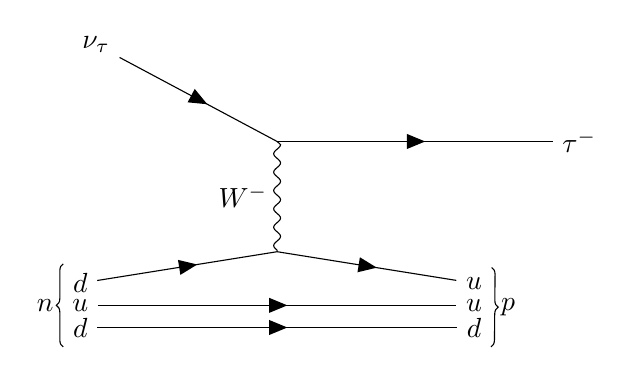
\begin{tikzpicture}
\begin{feynman}
\vertex (d1) {\(d\)}; 
\vertex[right=5cm of d1] (u3) {\(u\)}; 
\vertex[below=0.8em of d1] (u1) {\(u\)}; 
\vertex[right=5cm of u1] (u2) {\(u\)};
\vertex[below=0.8em of u1] (d2) {\(d\)}; 
\vertex[right=5cm of d2] (d3) {\(d\)};
\vertex[above right=0.4cm and 2.5cm of d1] (v1);
\vertex[above=1.4cm of v1] (v2);
\vertex[above left=1cm and 2cm of v2] (nu) {$\nu_{\tau}$};
\vertex[right=3.5cm of v2] (e) {$\tau^-$};
\diagram* { {[edges=fermion]
(d1) -- (v1) -- (u3), (u1) -- (u2),
(d2) -- (d3), (nu) -- (v2) -- (e)},
(v1) -- [boson, edge label=\(W^{-}\)] (v2)
};
\draw [decoration={brace}, decorate] (d2.south west) -- (d1.north west) node [pos=0.5, left] {\(n\)};
\draw [decoration={brace}, decorate] (u3.north east) --  (d3.south east) node [pos=0.5, right] {\(p\)};
\end{feynman} 
\end{tikzpicture}
\begin{tikzpicture}
\begin{feynman}
\vertex (a) {\(\tau^{-}\)};
\vertex [right=of a] (b);
\vertex [above right=of b] (f1) {\(\nu_{\tau}\)};
\vertex [below right=of b] (c);
\vertex [above right=of c] (f2) {\(\overline \nu_{e},\overline \nu_{\mu},\overline u\)};
\vertex [below right=of c] (f3) {\(e^{-},\mu^{-},d\)};
\diagram* {
(a) -- [fermion] (b) -- [fermion] (f1),
(b) -- [boson, edge label'=\(W^{-}\)] (c),
(c) -- [anti fermion] (f2),
(c) -- [fermion] (f3),
};
\end{feynman}
\end{tikzpicture}
\end{center}
The software that was written has a couple of shortcoming that could be fixed:
\begin{itemize}
    \itemsep-1em
    \item \textbf{Secondaries}: In the picture above, one can see that this process results in 2 neutrinos for every tau decay. Right now, we only track the leading $\nu_{\tau}$.
    \item \textbf{IceTray Interface}: We would like to get this code to play nicely with IceCube software to incorporate it into future collaboration analyses
    \item \textbf{New analysis}: Ultra-high-energy $\nu_{\tau}$ from cosmogenic fluxes (proton interactions with the CMB) \cite{Greisen:1966jv, Zatsepin:1966jv, Allison:2018cxu, Ahlers:2010fw, Ahlers:2012rz, Heinze:2019jou, Murase:2015ndr, Murase:2014foa, Fang:2013vla, Boncioli:2018lrv, Biehl:2017hnb} should also cascade in energy like this and might be detectable by IceCube
\end{itemize}

\subsection*{\textbf{Fast Radio Bursts}}
The enigmatic radio transients, Fast Radio Bursts \cite{Lorimer:2018rwi, Keane:2018jqo} have been predicted by some to emit neutrinos \cite{Li:2013kwa}. Some previous analyses have been performed \cite{Aartsen:2019wbt, Aartsen:2017zvw, Fahey:2016czk}, but there are other channels to look for this signal (cascade events, low energies), and the number of detected FRBs has increased dramatically, so stacking with the increased statistics could help.

\subsection*{\textbf{Fast Response Analysis}}
To rapidly respond to interesting astrophysical transients, we maintain a framework to quickly analyze IceCube data. In addition to running the actual analysis, we need help monitoring different outlets to find out if there are any sources worth following up.

\subsection*{\textbf{Radio-$\nu$ Correlation}}
Abhishek has begun an analysis to see if there is a correlation between neutrinos and radio-loud AGN, looking both for correlations with sources that are on average radio bright as well as for correlations with individual radio flares. There are various hypotheses to test, and many hands make light work.

\subsection*{\textbf{Source Number density constraints}}
A diffuse flux of neutrinos has been detected, but sources haev yet to be identified. One question to ask is: are there a few bright neutrino sources that create this flux or is it many dim sources? By looking in directions where you are confident there are neutrino sources (ie in the direction of our highest energy events), you can look for additional events to answer this question. We are working on a short timescale version of this, and plan to scale to longer timescales in the near future.

\subsection*{\textbf{Gravitational Waves}}
Raamis has been working on trying to find joint sources of gravitational waves and neutrinos. Right now, the analysis is focused on high energy tracks over short timescales. Possible future analyses include longer timescales, lower energies, and cascade event selections. 
\chapter{March 3, 2020}

%\section{Open Topics}

\subsection*{\textbf{Tau regeneration and GZK}}
Ibrahim reviews the problem: interactions nearby but outside the detector did not have all decay products tracked, and some muons came out backwards. When looking at muons that make it to final event selection, contamination at higher energies reaches upwards of 20\%. A new simulation set was submitted via simprod. Plan is to give an update and introduce the GZK analysis on a diffuse call in a few weeks.

\subsection*{\textbf{Computing Needs}}
Upcoming Scientific Computing Advisory Panel (SCAP) review: 
\begin{itemize}
    \itemsep-1em
    \item NPX has been slow (over 50,000 idle jobs right now)
    \item Disk system has been somewhat unreliable over recent years, more stable lately
    \item Over the last year or so, the number of users tanking the cobalts has decreased
    \item Not many cores on the \texttt{realtime} machine, makes some jobs slower to run on realtime machines although they tend to be more stable because few people use the machine
    \item Problems with alert event scans killing GPUs
    \item Carlos is happy with \texttt{cvmfs} over the last few years, especially building user specific \texttt{cvmfs} things
    \item wiki page search doesn't work
    \item increased documentation (SkyLab specifically)
    \item It might be helpful to assign someone to work on Memory leaks as s service task
\end{itemize}

\subsection*{\textbf{Novae}}
Brian Metzger requested a plot for a 1-10 day timescale sensitivity for a novae white paper. Might want to decouple a public effective area (maybe from Mia's or Jason's recent conference talks?) and a more in depth longer timescale Upgrade or GRECO sensitivity (either through the collaboration or otherwise)

\chapter{March 10, 2020}

\subsection*{\textbf{Tau regeneration and GZK}}
Ibrahim showed $\nu_{\tau}$ effective areas for the diffuse $\nu_{\mu}$ selection, and at 100 TeV they are about 25\% the effective area for $\nu_{\mu}$. It does look like there might be a bit of a problem with flattening at higher energies that Carlos thinks shouldn't be there. Discussed checking to see if MEOWS or diffuse $\nu_{\mu}$ is more sensitive to this. Manuel is giving a talk in diffuse, we recommended he doesn't mention any of this stuff

\subsection*{\textbf{FRB paper typo}}
ping Ali again, encourage him to reach out to ApJ.

\subsection*{\textbf{Gravitational Waves}}
One week into collaboration review, no comments yet. Raamis will reach out to Zsuzsa for LIGO review. New ANTARES paper on O2 followups \cite{Molla:2020wsw}.

Cascade analyses show a large spike for the most negative TS value, because the rate for the cascade sample is much smaller than that of GFU. Preliminary sensitivities are fairly consistent between the two samples, but some questions to look into include whether or not this is all flavor or per flavor.

I suggested recreating Figure 1 from the GW paper but for the cascade sample to see if the intersection occurs right towards the median of the declination of GW150914. Fits are \textit{suspiciously} perfect, maybe just as a consequence of short timescale. Suggested to push out to larger time windows. Might also be worth it to calculate the fit $n_s$ at the location of the injected source, not just on the whole sky. Fits of $\gamma$ are inconsistent with the injected $\gamma=2.0$

Next step is to include fluctuations in rates. Test would be to calculate median significance for parts of the year when there are maximal and minimal rates using both the all sky method and the declination band method. 

\subsection*{\textbf{Abhishek: Number of sources}}
Abhishek has looked into Eddington Bias. Looked at plot from Eddington bias paper \cite{Strotjohann:2018ufz}. Discussed including poisson fluctuations to map from flux to number of events and then sample from there, not just rescaling the sensitivity in flux space. Justin recommended interpolating the sensitivity curve (in terms of number of events) to get what it would be for a $\gamma = 2.5$ and then comparing poisson fluctuated number of events for each source to that to calculate the number of detected sources. 

For blazar analysis, problem with mismatching hypotheses with likelihoods is fixed. Abhishek also shows overlap between MOJAVE and 3FHL source samples. Ibrahim suggested a scatter plot of radio flux and gamma-ray flux for the different samples. In some of these plots it might also be nice to compare to the total fraction of diffuse.
\chapter{Visualizing the source density phase space}
With the measurement of a diffuse neutrino flux but uncertainties in the astrophysical origins, one can ask if the dominant source class which produces neutrinos are \textit{rare and bright} or \textit{numerous and dim}. One way to do this is by looking for point source excesses. With the lack of any clear point sources, neutrino bright objects can be excluded, and thus attributing the entire diffuse flux from steady, rare ($<\mathcal{O}(1\; \mathrm{Gpc}^{-3})$) objects can be excluded with current limits. The effective source densities which can be probed change significantly with a detector like Gen2. All of this is normally visualized in Figure~\ref{fig:current_fig} (Figure taken from \cite{Aartsen:2019swn}).

\begin{figure}[h!]
    \centering
    \includegraphics[width=0.45\textwidth]{images/continuous_Gen2_revised.pdf}
    \caption{Comparison of the diffuse neutrino flux (magenta) to current and projected point source sensitivities (blue lines), as well as the effective local source density and luminosity of various candidate source classes.}
    \label{fig:current_fig}
\end{figure}

A quick notes about the figure: making an argument such as ``x\% of source class y could still explain the diffuse flux'' is true if the star corresponding to source class y, when moved down on the y-axis by the appropriate ratio, is below the point source limits.

This way of visualizing the parameter space downplays the large region of parameter space the Gen2 could probe. Also, it is the transpose of what you might intuitively do, as luminosity is somewhat analagous to flux, which we plot vertically and forbid regions above (not to the right of) limits. Additionally, even under the assumption that numerous source classes contribute to the diffuse flux, there are likely only one or a few that contribute at a greater than 10\% level, and these are the real targets of searches in this spirit. As a result, the true parameter space of interest is not as large as this plot would lead you to believe. 

Some suggestions for improvement include transposing the plot and possibly hatching the part of the parameter space that explains 100\% of the diffuse flux once we have gen2, as is pictured in Figure~\ref{fig:transposed}.

\begin{figure}[htb]
    \centering
    \includegraphics[width=0.48\textwidth]{images/lumi_density_rotated.pdf}
    \includegraphics[width=0.48\textwidth]{images/lumi_density_hatched_rotated.pdf}
    \caption{Transpose of the previous figure, so that higher luminosities are found by moving vertically upwards in the plot}
    \label{fig:transposed}
\end{figure}

This plot still has the problem of presenting a lot of uninteresting phase space (bottom left). To remedy this, we could plot $\rho_{eff}\times \mathcal{L}_{\nu}$ on the vertical axis, in much the same way that power law spectra are scaled by powers of $E_{\nu}$. Doing this results in Figure~\ref{fig:scaled_lumi_density}.

\begin{figure}
    \centering
    \includegraphics[width=0.48\textwidth]{images/lumi_density_product.pdf}
    \includegraphics[width=0.48\textwidth]{images/lumi_density_product_hatch.pdf}
    \caption{Luminosity times effective local density plotted on the y-axis to focus on the interesting region of parameter space.}
    \label{fig:scaled_lumi_density}
\end{figure}

One nice consequence of this visualization is suppose you have a candidate source class that could produce a fraction, $f$ of the diffuse flux. Then (ignoring uncertainties on the diffuse flux), this just corresponds to moving down in the plot by a factor of $f$ from the vertical magenta line. This is shown in Figure~\ref{fig:diffuse_fraction_lumi}. 

\begin{figure}[h!]
    \centering
    \includegraphics[width=0.5\textwidth]{images/lumi_density_fraction.pdf}
    \caption{Similar figure as above, scaled by the diffuse flux to highlight interpretation.}
    \label{fig:diffuse_fraction_lumi}
\end{figure} 


\chapter{March 31, 2020}

\section{O3 is dead}
\subsection{Long live O3}
Raamis will incorporate documentation for how to run GW code into an appendix of his thesis. I will work on bundling up latency stuff with Raamis's code so that it shouldn't be hard to turn back on. 

Also talked about hosting GW results on the ROC internal or external server. 

Also maybe having O4 cascades run in realtime even if Raamis graduates before then.

\section{AAS and APS planning}
Four contributions at AAS (Justin, Raamis, Abhishek, Me) and two for APS (Me and Justin).
For APS, Justin might want to update to the full O3 table of followups, for ANITA it should pretty much just be the ICRC slides.

Discussion later this week on whether or not we will send slides around to neutrino sources or just present because compiling GW plots could be a bit riskier.

\textbf{Neutrino 2020 planning}: Maybe GZK analysis if Ibrahim makes substantive progress in the next 2 weeks

On a serious note, talked about maybe submitting abstracts for everyone (ANITA, GW, FRA). Nothing definitive decided.

\section{$\tau$}
Ibrahim will be talking on the Diffuse call at 4:30 tomorrow about the secondary GZK analysis and discussing the bugs he unearthed. 

Also showed distributions in Truncated energy for both $\nu_{\tau}$ and $\nu_{\mu}$ for an injected $E^{-1}$, as well as comparisons to analytical expectations for effective area. Plot looks really promising, but Carlos mentioned some reasons for small discrepancies (geometric area vs. muon effective area, neutrino vs. average neutrino antineutrino).

Please look over Ibrahim's slides before tomorrow, specifically the zenith angle distribution plots. 

\section{Abhishek}
Abhishek compares the MOJAVE sample to some other samples used in other IceCube analyses. There's a decent amount of overlap between the IC86 blazar stacking analysis and Tessa's 10 yr point source. Only 2 overlapping with the ULIRG stacking, and only 56 from the RLAGN search (which has 13927 sources to start with).

For MOJAVE, there are memory problems when stacking many sources, I will help to take a look at this. 

Justin suggested a scatter plot for the common sources.

Justin and Ibrahim were a bit surprised at the low number of overlapping sources with MOJAVE and the RLAGN analysis (maybe because RLAGN is designed for off-axis?) 


\section{FRA}
Might be nice to see the background expectation too in addition to the ratio of 100 signal events when comparing to the alert event effective area. 
\chapter{April 7, 2020}
\section{\texttt{TauRunner\_v2}}
Ibrahim implemented some options that make checking with \texttt{nuTauSim} a lot easier, including: options to add ice layers as well as change between dipole and perturbative QCD cross sections. He also fixed a minor bug that was always reporting tau energies at decay instead of possibly upon exit, he fixed this, and is running some jobs to cross-check previous results (shouldn't change much). Nepomuk's student at Georgia Tech is comparing the two frameworks, which initiated these comparisons. 

Justin and Carlos suggest putting some plots together and putting them on the repo to highlight the fact that \texttt{TauRunner} is self-consistent. Carlos also pointed us to the IceCube Earth Models.

For the diffuse analysis, Ibrahim is looking at MEOWS effective areas. Almost at the point where Ibrahim might need to attach the simulations. Carlos wants to add the patching as \texttt{LeptonWeighter} functionality. 

Diffuse call went well, WG is happy that people are looking into $\nu_{\tau}$ simulation, and the diffuse $\nu_{\mu}$ group is looking at including these. Brian clark also mentions non-GZK EeV sources (extreme EeV neutrino point sources). 

\section{Gravitational Waves}
Raamis submitted to arXiv yesterday and is waiting to give Maddie the okay for the news article. Raamis will submit to the journal and send the arXiv password to the review committee. Acknowledgements don't include any named authors or institutions, Raamis will ask Segev who to name. Raamis is working on updating the full table with results from O3b and needs to calculate all new $E_{\mathrm{iso}}$ upper limits (some O3a needed to be rerun after the radians bug).

Raamis is also working on APS slides. He also reached out to Ali about reviewing, no response yet.

\section{Radio stacking}
Abhishek compares weights from sources that are in his analysis and other analyses. Suggestion to change ``IC86'' analysis to something like 2FHL. Question came up about why Federica excludes a band around the Galactic plane (does this account for the sources in Abhishek's catalog that are not in Federica's? Abhishek says it does for about 50). Ibrahim says that Federica weights by x-ray and IR which do extragalactic catalogs.

Abhishek compares to a recent paper from authors not affiliated with IceCube that looked at VLBI sources. Justin suggests comparing to their full source list if possible. Plavin et al. uploaded a new version this week, might be worth checking to see if any claims in the paper changed.

Will also include injecting $E^{-2.5}$ and start working on fit vs. injected plots.

\section{Fast Response}
I'm running steady trials for 8 years of GFU data on two years of alert events. Switched over to the 2 year of v2 alerts being shared with GBM. Need to figure out how to map from LLH to PDF, will reach out to Claudio for this. Also working on answering Theo's questions, Carlos suggested modifying the $\Delta LLH$ to include a correction term for low statistics exceptions to Wilk's.

\chapter{April 21, 2020}
\section{Conference planning}
\textbf{APS}: Interesting talks: GW190412 overviews, Abhishek recommends AMEGO talks, CHIME FRB talk (up to several hundred, upgrade plans for better localization)

\textbf{AAS}: Registration is due today, unsure if we have talks or posters yet, but still have to confirm that we will be attending. Should we change procedure for AAS based off of GW-Columbia interactions for APS. Planning on similar GW talk for AAS, but maybe will go through full approval process (not necessary, but could be nice to do). For novae, would be nice to get a full differential sensitivity curve similar to the ones we want to show Brian. For Abhishek, maybe targeting plot approval of sensitivity curves. Goal is to have plot approval ready for parallel talks during the collaboration meeting

\textbf{Collaboration Meeting}: Talk requests due a week from today. Plan: Raamis on O3 wrap-up (maybe plenary?) / plots for approval and a cascade talk (maybe a two-week contribution as well), Ibrahim in diffuse for GZK and submitted abstract to Pheno 2020, Alex on number density and novae during collaboration meeting and externally triggered on nu-sources next week, Abhishek on radio and maybe on source number density (gong?)

\textbf{Neutrino 2020}: Novae stuff might get put in the other GRECO contributions (Chujie and Michael). Two ANITA contributions, submit collaboration paper abstract to icecube-c by this Friday for submission by next friday to the conference, also encouraging Raamis and Abhishek to submit abstracts. Plot approval is necessary for Neutrino. 

\section{$\tau$ and GZK}
Joran updated fit to include new MC, and the diffuse numu fit is already softer (2.38) before even adding taus. Ibrahim is working on completing the MEOWS simulation. Goal is to redo fit with just a nutau astrophysical component by the collaboration meeting. Fits on MEOWS will just be on realizations.

Email from NuPropEarth authors, mainly Alfonso, comparing TauRunner to NuPropEarth. Pretty good agreement right now, despite different implementations of earth layers, cross sections, etc. Might be a good idea to just look at the secondaries and ask the NuPropEarth folks to show distributions of just secondaries (like we did in the few author paper). 

Ibrahim added an Earth Module so that users can tweak the number of layers used. Hallsie and Romero-Wolf requested some numbers for comparison.

\section{Gravitational Waves}
Updated version of $E_{\mathrm{iso}}$ upper limits with O1, O2, and O3 mergers. Suggestion to add "GW candidates with distance estimates" to clarify why the unmodeled burst is missing. Hypothesis: scatter due to declination distribution, maybe make a plot with $E_{\mathrm{iso}}$ with centroid declination. Maybe make gamma-ray point orange. 

Raamis shows a check between the full calculation and a back of the envelope without the full marginalization, and overall there is pretty good agreement. Also shows a p-value distribution. I suggested sampling from the bg TS distributions to create what the expectation actually looks like. Also has a comparison of the 90\% error regions of GFU events compared to GW localizations. Will double check this plot for the floor implementation. Justin suggests also showing what it would look like for signal too. 

For cascades, unable to reduce bias in fitting the spectral index. Raamis is looking into this.

\section{Radio correlation analysis}
Compared to the recent Plavin et al. paper. Justin asks about eventual quantitative comparison, Abhishek isn't sure because they didn't report such a number. Abhishek compares all of the sources that have been mentioned in IceCube followups in the last few years. 3 of the 4 sources from the $k=4$ in Tessa's analysis are in the sample, NGC 1068 is the one that is not.

Abhishek also shows his bias tests for recovering injected signal with an injected $E^{-2}$. He also discusses his plans for how to calculate completeness.

\section{Fast Response and Novae}
Discussed comments with Theo, he is happy. Moved webpage to the roc website. Will try to talk on nu-sources this monday with just a short update of the externally triggered work so that I can dedicate my collaboration meeting talk to following up the IceCube alert events. Working on what to do with the skymap areas, thinking of just using the normalized likelihood maps. Paper plans: two separate or one big one?

For novae, working on differential sensitivity curves as well as standard 10 day sensitivity curves

\chapter{April 28, 2020}
\section{Conference planning}
Neutrino abstracts circulated to icecube-c, submit by this Friday. AAS confirmations by last week. Send drafts of collaboration meeting slides internally by this Friday, we may or may not have heard definitively about talk assignments by then. As of now, we will plan to hold our normal Tuesday meeting next week. Ibrahim is giving a talk at Pheno next Tuesday. 

\section{$\tau$ (Ibrahim)}
Ibrahim working on LeptonWeighter to do the weighting for the leptons, just be able to reuse the muons simulation that's ready. Preliminary checks are promising, but plots to come in the future. Ibrahim has a set of neutrinos through the normal simulation chain as well. Estimate is a few $\mu$ from $\nu_{\tau}$ above 100 TeV in 10 years of data assuming a certain spectrum. Asimov sensitivities to come after that. 

\section{Radio Correlation (Abhishek}
Some fighting with the cluster, but Abhishek has fitting tests for different injected spectra. Some jumpiness in the softer spectra, might be statistical. Justin suggested looking at the actual spectra instead of just the flux at a certain energy, maybe in the same fashion as Mehr in her recent nu-sources slides.

Abhishek also has some overlays with comparing to the fraction of the diffuse flux. Numbers seem a bit overly constraining. Abhishek is also going to look into what he needs to do with tech leads to get his code approved.

\section{Gravitational Waves (Raamis)}
Raamis made a plot of $E_{\mathrm{iso}}$ vs. the centroid declination. Doesn't seem to be much of an trend (maybe slightly negative slope, consistent with what you might guess). Justin suggests plotting the residuals of the distance plot, to see if the additional scatter in the $r^2$ plot is due to declination.

p-value distribution: Raamis did a KS test with both a uniform distribution as well as actually sampling from the p-value distributions. Double checked that the definition of the figure of merit in the KS test comparison, 

\begin{equation*}
    D_{n m}>\frac{1}{\sqrt{n}} \sqrt{-\frac{\ln \left(\frac{\alpha}{2}\right)\left(1+\frac{n}{m}\right)}{2}},
\end{equation*}
properly handles the sample size. Justin suggested doing a $\chi^2$ test as well.

For cascades, Raamis looked into the gamma fits. Some weirdness with finding local minima, I suggested plotting with $n_s$ fixed to the maxima, not truth, or maybe making a 2d LLH scan with both parameters. Actual fitting vs. injected signal plots with cascades look \textit{weird}. Justin suggests sending some of this to Steve or Mike to see if they have helpful input.

Carlos brought up a discussion on justifying the $E^{-2}$ spectral assumption for the upper limits. We discussed different approaches, such as doing it for different spectra or creating differential sensitivities. 

Raamis is on the analysis call for Thursday to request plot approval. Justin had some suggestions on the plots:
\begin{itemize}
    \item $E_{\mathrm{iso}}$ vs. distance plot: events and candidates consistency, candidates should be singular for the cbc. Period for last sentence.
    \item p-value distribution: Title changed to candidates. Borderline fontsize. Justin suggests adding the one with the sampled background distribution as well. 
    \item For the GW vs neutrino localizations, switch to just one. Justin thinks maybe the signal one makes sense. Might make sense to make equal sized bins in log-space (Raamis will look into this though because aesthetically it might be hard). Justin also suggests avoiding ``GFU'' in favor of ``IC'' or something of the like.
    \item Latency plot: maybe decrease sig figs in legend. Make sure there is a space between number and unit
    \item Skymaps: Increasing the title font size. 
    \item Zoomed in plots: increase font size, add fourth for completeness, maybe include full sky maps nearby as references
\end{itemize}

\section{Fast Response and Novae (Alex)}
I showed some stuff.

\chapter{May 5, 2020}
\section{Virtual Collaboration Meeting: plans and progress}
\subsection{Gong Talks}
\textbf{Raamis Cascades (3:45):} Justin suggests that it might be nice to have some skymap sensitivity comparison on the point source sensitivity plots. Justin has a pet peeve about using ``ideal.'' Be explicit about flavor. Mention on slide 2 that it's $E^{-2}$. Specify discovery level on slide 3. Long term also want O3. Might want to emphasize that this sensitivity is flatter further out than you get with GFU. Specify that it's Mike Richman's sample in the beginning. Raamis will send .ppt source to Doga and follow up with him if he doesn't send a draft soon.

\textbf{FIRESONG simulation (4:10):} Justin requested larger fontsize. ``Blazar'' sources is redundant, and it doesn't have to blazars, so it can just be ``sources''. Emphasize that the construction is as conservative as possible in the first slide. Text too small on slide 2. Maybe mention standard candle on slide 2. Maybe mention that it doesn't account for Eddington bias. Remove ``number of'' in first bullet on slide 3. Remove last column from table. Extra time could be used to talk about breaking the degeneracy between the low density and high density number of detections.

\subsection{Parallel Talks}
\textbf{Radio-AGN connection:} Maybe change title to ``Search for'' or ``Test for'' correlation. Correlation will help us $\rightarrow$ correlations would help us. Include slide numbers. Slide 6: inconsistent capitalization of MOJAVE. Might be nice to include the $E^{-3}$ as well, might want to specify injection is matching the hypothesis going into the weights. Just call the blue sensitivity. Orange line has the wrong power law. Abhishek will fix this and send around a new version when he has it. Fixed version: remove bottom panel and quote fixed factor

\textbf{Novae:} Mention the spectra on slide one are from Anna's paper. Double check stacked result from Anna's paper. Maybe include the Brian quote in intro slide. SLide 5: subscript ns, slide 8: converting to scaling. Slide 9: mention all flavors or add the factor, change legend to GRECO, DeepCore. Slide 10: allows us. Add bullet about hoping to show some of these plots at Neutrino and AAS. Look into timeline for plot approval

``More than likely we will need Gen 2 and a lot of luck (e.g. a very nearby nova) to detect a signal, but I have enough faith in the hadronic model that [it] is a pretty sure bet it's there.'' — Brian Metzger

\section{Gravitational Waves (Raamis)}
Raamis will forward reviewer comments to the committee, he talked about some of the reviewer's comments. 

\chapter{May 12, 2020}
\section{Doga's plenary slides}
Raamis took notes for this part

\section{Paper outline}
\begin{itemize}
    \item Remove extreme from title and abstract
    \item Remove premier in abstract (maybe unique or just remove)
    \item realtime pipeline instead of realtime data or low-latency data
    \item analyses to followup analyses
    \item analyses performed to YY date
    \item synonym for pipeline in abstract
    \item Maybe switch sections 3 and 4
    \item Likelihood Analysis to Analysis Method
    \item Maybe move appendices to results
    \item 2 calendar years (ie 11-12) in legend, seasonal fit -> ``sinusoidal fit.'' Add a comment about the north vs. south. Maybe include some more information about the seasonal fits in the appendix or just in the main body.
    \item Remove 50\% in legend
    \item Figure 2: Move to the 90\% CL for, more xticks, consistent units and expressions in axis labels, too much space between DeltaT and ``s.'' Figure 4: maybe dotted between bins. Figure 3: Make the light gray darker
    \item Figure 5: $\log_{10}$, captial Delta T, maybe start caption with more qualitative sentence: ``Statistical significance expected when detecting one event.''
    \item Add a paragraph in the text about why the p-value distribution has the peak
    \item Results table: Remove ``all'' in second sentence, ``and constrain''. Source names, add a type column in the table.
    \item Maybe make some of the back of the envelopes into plots for the discussion section
    \item Maybe change colormap for zoomed skymap
\end{itemize}

Maybe make an event view for the really weird event, maybe make some histograms of 50\% containment and stuff

\chapter{May 19, 2020}
\section{AAS and Neutrino Planning}

\section{Gravitational Waves}
Raamis updated the paper with reviewer comments and a small one from me. Paper includes updated $E_{\mathrm{iso}}$ plot with the PS band. Raamis will work on preparing an official response to the reviewer. News article looks good.

Even with sparser binning things look a bit off, but less so at shorter timescales.

\section{Abhishek}
Abhishek is seeing some disagreement between his calculations and previous stacking analyses by about an order of magnitude (Abhishek's seem too constraining).

\section{Taus}
Came to a consensus that we don't really have anything to share with Stephanie. Maybe pitch the idea of a joint analysis?

\chapter{May 26, 2020}
\section{AAS Slides}
\textbf{Abhishek}:
\begin{itemize}
\itemsep-1em
    \item add ``for the IceCube Collaboration''
    \item tweak the title to make it less general
    \item Include affiliations on title slide
    \item Tweak language on slide 6: ``perform a time-averaged source for . . . '' to emphasize the relationship is a part of the hypothesis
    \item Remove histogram from slide 6
    \item Ideally there would be an error band for the diffuse flux (like the butterfly) over the proper energy band
    \item 3fHL has a small f in the legend
    \item Some discussion about the placement of the different lines on the sensitivity plot
    \item Simplify last bullet on slide 7 (don't mention blinded or preliminary)
\end{itemize}

\textbf{Raamis}:
\begin{itemize}
\itemsep-1em
    \item Raamis shows some plots from running various signal injection trials
    \item Promising results with a spatial only likelihood. Raamis is going to look into this a bit more systematically and submit a whole bunch of jobs to test this
\end{itemize}

\chapter{June 23, 2020}
\section{$\tau$ and GZK (Ibrahim)}
Trying to schedule a meeting with Stephanie. Topics for discussion: Why we don't have their effective areas, trying to figure out the scale of the project (size of the group, general PS versus following up ANITA-IV).

Analysis progress a bit stalled, Ibrahim is working on running the new jobs on the new computing cluster through Harvard. Right now, Aachen is not including the separate $\tau$ component in the fit.

\section{Gravitational Waves (Raamis)}
Paper was accepted to ApJL, Imre reached out about adding acknowledgements during proofs. Raamis got the greenlight to move forward with the two week timescale analysis from his reviewers. Cluster has been down, so not all precomputed jobs finished. For cascades, there are still some items on the to do list for looking at the fits. Raamis working on making all of the relevant plots for the same time windows as tracks. He will get a slot on an upcoming call.

\section{Radio stacking and sensitivity scaling vs. source density (Abhishek)}
Cluster failures are holding up Abhishek. Abhishek is working on using Christoph Raab's lightcurve code, but there are some problems with python2 vs. python3 compatibility. Justin suggested comparing to something that might be related, where instead of using the lightcurve as a temporal term in the signal PDF, stacking independent observations, treating different time windows as different sources, and stacking those observations together. We talked a bit about if the likelihoods are equivalent, but aren't quite sure one way or the other.

\section{Fast Response (Alex)}
Showed some plots with updating the full 2d luminosity-density plane for 3 different transient time windows (1000 s, 2 days, 31 days), and for the time integrated case

\section{Novae (Alex)}
I showed a comparison of some LE event selections (GRECO, OscNext, Upgrade, ORCA). Some questions about Upgrade, I may reach out to Tom with any questions

\section{Gravitational Waves with GRECO (Aswathi, Raamis, Alex)}


\chapter{June 30, 2020}
\section{Radio stacking (Abhishek)}


\section{Gravitational Waves (Raamis)}
Raamis about to resubmit the paper (got the okay from Segev for acknowledgements). Ali is the WG reviewer for the cascades analysis. No word back from Anna about the analysis call for the two-week search. Discussed a bit about the ZTF optical counterpart, which Raamis is working on including in his unblinding request. Raamis working on the cascade wiki, where he'll put the info for fitting the index

\section{Fast Response (Alex)}


\chapter{July 7, 2020}
\section{$\tau$ and GZK (Ibrahim)}
Ibrahim talked with Stephanie during his poster session. They think that the effective areas we used in our paper were possibly not accurate, she would like to do a rigorous comparison between our effective areas, with similar cross sections and such. They also talked about possibly doing a subthreshold analysis looking into the south pole masking in the ANITA analysis. Aswathi mentions that it might be hard to disentangle any signal from the direction of the ICL over the large constant background.

Ibrahim offered to make a set of slides explaining what we did in the collaboration paper for the effective area to spell out everything. 

For the GZK analysis, they need to add the splines to GolemFit. Ibrahim is planning on meeting with Jeff to discuss how to run the necessary monte carlo sets. Plan to revisit discussion with Shigeru after they get sensitivities (WG leads seemed confused by some of Shigeru's argument)

\section{Radio stacking (Abhishek)}


\section{Gravitational Waves (Raamis)}
Finished running fit and injection tests. Index is a bit soft, recovered signal looks good. Reran sensitivities for a few events, there's an order of magnitude improvement for $E^{-2.5}$ with 7yr MESC vs. GFU when looking at GW150914. Working on finishing up the same comparison for GW170608. Justin suggests running cascades for all 3 available events (can only do O1 when it's time to run because of the date range of MESC).

For the localization comparison plots, Raamis has median and 90\% plots, and will rerun the MC ones with weighting the MC event according to an $E^{-2}$ spectrum. Running jobs for 2 week events, analysis currently in collaboration review. Justin suggests making a fixed request for the optical counterpart and proposing that. Raamis received second set of proofs for the paper this morning. 

\section{Low energy GWs (Aswathi)}
Aswathi found some relevant papers about GeV neutrinos, most are about BNS or BHNS mergers with GRB progenitors. 

Aswathi already has effective areas. We discussed why the curves decrease at higher energies, and it might be related to reconstructions failing for high charge events, but it looks smooth up to about 10 TeV. Justin suggests speaking on one of the upcoming GRECO calls. 

Carlos mentioned an SLC bug that Tom is presenting on the Tuesday call, which could affect our analyses.

\section{Fast Response (Alex)}
Fix the time windows

SLC hits Bug (Tom): There was a bug found in the SLC hits for simulation. It was traced to a bug in DOM launcher that results in a one bin offset in simulation by 25 ns (not in data). Preliminary checks to see if there were major changes. There were shifts in the reconstructed zenith angle distribution (fairly significant). Might be a shift from upgoing to downgoing and high energy to low energy systematically. This only affects monte carlo, but seems like a noticeable affect in monte carlo. As of yesterday, there is a new genie set with a bug fix, should expect a more detailed explanation soon. 

\chapter{July 14, 2020}
\section{Radio stacking (Abhishek)}
Abhishek has been looking into what Stefan Coenders did in his scripts to see if he can get the same results with his data. Some higher stats might be necessary to flush out the full error band

\section{Gravitational Waves (Raamis)}
 

\section{Low energy GWs (Aswathi)}


\section{Fast Response (Alex)}

\chapter{August 25, 2020}
\section{Lightcurve stacking (Abhishek)}
Abhishek is trying to combine some of Christoph Raab's code with some code that Raamis and I have written. We talked about some of the objects in Skylab that make the most sense to use for a lightcurve based analysis. Qinrui has experience with both Skylab and csky based lightcurve analyses, so Abhishek will likely discuss with her about some of the technical details.


\section{Gravitational Waves (Raamis)}
Raamis finished his upper limit calculation for the 2 week unblinding. He is working on S190910h differential upper limit. Ready to request a slot on the nu-sources call to present unblinding results, but if it looks like the differential UL won't take long, then Raamis says it makes sense to wait and show all of it.

Raamis also showed a comparison between the TS from using a GW skymap with one pixel localization to using the point source implementation, and the TS values agree for a variety of background trials. For signal injection trials, there are small disagreements with the trials that are not very significant. I asked if it's related to the pixels that are being looked at because of the ``pixel scan'' function, and Raamis said he was wondering the same thing and will look into that. Aswathi asked about the negative infinity convention, and we also discussed whether or not the pixelization method is a grid of points or true pixelization. For cascades, Raamis is working on reproducibility requirements and answering some of Ali's questions 
 

\section{Low energy GWs (Aswathi)}
Aswathi showed the results of increased statistics fit bias tests. We discussed some technical questions about the skylab prior injector. Overall, it looks promising that you can do an analysis with the full GW localization and the poor event reconstructions from GRECO. 


\section{Fast Response (Alex)}
Transient background and signal injection trials for the alert event follow up are done, and I showed the BG TS and ns fit bias distributions from these trials. I also showed some distributions of the alert events (signalness, declination). There are 249 alerts, 2 different time windows, and the option to include or ignore systematic smearing of skymaps, so all things considered there are about 1000 different sets of background and signal injected distributions. I showed some summary plots of these distributions (as well as panel plots of all of the distributions, sorry for all the plots), and things look as they should, but I noticed some failed jobs and some weird sensitivity values that I'm double checking. I also automated the cascade followup, and it's running in realtime (on scrambled data) to test the pipeline.
\chapter{Realtime Bootcamp, September 2020}

\section{Erik: Overview talk}
\begin{itemize}
    \item Overview of alert streams: SNDAQ, GFU/OFU, alert events, Fast response, realtime GW
    \item Single neutrino track alerts: $\mathrm{signalness} = \frac{N_{sig}}{N_{sig} + N_{bg}}$
    \item Details on streams in a document on the GCN server
    \item Estimate of around 30 track alerts per year and 8 cascade alerts per year
    \item Walked through online filtering
    \item For info on how to log in and become the followup user, run \texttt{sudo su - followup} while on the \texttt{followup-*} machines
    \item Walked through one of the listener scripts together
    \item Note the hierarchy of check GFU first, then EHE next, then HESE after that
\end{itemize}

\section{Cristina: Millipede Scans}
\begin{itemize}
    \item Overview of the pipeline
    \item Discussed how to estimate time remaining and the messages that ``Marvin'' sends
    \item Sample GCN circular
\end{itemize}
\chapter{September 22, 2020}
We discussed moving our Tuesday timeslot, but didn't come to any conclusions.

\section{Alex: self-triggered alert followup}
I showed some updated luminosity / density constraints as well as a new fast response flux sensitivity plot (not time-integrated flux)

\section{Raamis: GW status}
Raamis showed his differential upper limit calculation.

Naoko asked why doesn't raamis just fix the index in the optical follow up because there is bias in the spectral fit. Assuming an $E^{-2}$ seems to be almost the same as floating the index.

Raamis also looked into what was weird with the double bump TS structure with the spatial prior analysis in GRECO, Raamis said he will discuss this with Aswathi offline

\section{Abhishek: MOJAVE and Fast Response}
Abhishek added a line with a completeness factor to the MOJAVE differential sensitivity. We discussed whether or not there is a physical and not observational definition of completeness for this sample.

Abhishek has begun running the fast response code as well. We discussed writing a latency page similar to the GW latency page that we had.

\section{Ibrahim: GZK and taus}
Ibrahim found a missing cut in his monte carlo processing scripts, so now the Monte Carlo weights are working, and he has a set of EHE in MEOWS and he added it to GOLEM-fit, and are getting about 1.4 GZK events in MEOWS. Ibrahim has also been looking into some populations of EHE point sources that he has been propagating. 
We went through his draft slides: Slide 2, maybe change right to $E \times d\Phi/dE$ instead of just $d\Phi/dE$, Slide 4 maybe add Github repo, Slide 5 add author names, Slide 8 umlaut with Joran's name

Ibrahim will send around the slides once the event distributions are finished.

Carlos also mentioned a technical paper comparing UHE tau tools.
\chapter{January 12, 2021}

\section{Gravitational Waves}
\subsection{High energies (Raamis)}
Raamis showed his unblinding results for the optical counterpart. Raamis is working on the background trials for the large time windows he needs for discovery potential. Some are still finishing, but the curve has the proper behavior of looking flat for very short times and then beginning to asymptote towards a square root scaling. In plot, blue line is the maximum livetime that we have for the event selection.

\begin{figure}[h]
    \centering
    \includegraphics[width=0.6\textwidth]{images/raamis_plot_011221.png}
    \caption{Optical counterpart discovery potential vs. time. Vertical line is maximum allowed livetime by dataset. He is working on the few remaining time windows}
    \label{fig:my_label}
\end{figure}

\subsection{Lower energies (Aswathi)}
Aswathi fixed the sensitivity efficiency curve plot!!

The problem was with a seed, where the same seed was getting used each time, and when the computation time was split up there were not unique seeds in each job. Aswathi shows both sensitivity as well as discovery potential. 

\begin{figure}[h]
    \centering
    \includegraphics[width=0.6\textwidth]{images/aswathi_plot_011221.png}
    \caption{Aswathi's fixed sensitivity efficiency curve}
    \label{fig:my_label}
\end{figure}

\section{Novae, Fast Response, Millipede Maps, etc. (Alex)}

I prepared fast response paper responses for ApJ and am waiting to hear back from the internal review committee.

I also reached out to Chad who said he would review the alert followup analysis and send questions in the next week or so.

Millipede maps were discussed yesterday on the call. The working group seemed happy about the interpolation, and Erik seemed happy about reducing the resolution to save the computation time. I will work on implementing this in the next few weeks.

For novae, I showed that I am having some problems at longer timescales, and I think it is from the low stats in the background distribution at long time windows. 

\begin{figure}[h]
    \centering
    \includegraphics[width=0.6\textwidth]{images/alex_plot_011221.png}
    \caption{Novae plot showing that the background distributions (bottom right) at large time windows suffer from low stats because of the collapsing BG TS behavior.}
    \label{fig:my_label}
\end{figure}

\section{Radio Stacking (Abhishek)}
Abhishek looked more into the differential sensitivity. Some of the files were being moved around a few weeks ago when Abhishek made the last version of the plot and so the monte carlo weights were messed up. Now that things are fixed, he recalculated the differential sensitivity and around 100 TeV the sensitivity is at the level of a few 10s of percent of the diffuse flux

\begin{figure}[h]
    \centering
    \includegraphics[width=0.6\textwidth]{images/abhishek_plot_011221.png}
    \caption{Abhishek's new differential sensitivity for radio stacking time-integrated}
    \label{fig:my_label}
\end{figure}

Abhishek is also working on calculating the central 90\% energy values for the single power law sensitivities.

Abhishek received questions from Federica and has responded to her and is waiting to hear back.

We also briefly discussed Abhishek's matrix of testing different hypotheses with the different injection schemes.

\section{ICRC Planning}
We discussed the ICRC planning and who will submit what topics. Topics to submit include:
\begin{enumerate}
    \item Aswathi: low energy GW
    \item Raamis: All high-energy analyses (tracks, realtime, optical, archival, maybe mention cascades). Could be broken up into a talk and a poster for current and upcoming
    \item Abhishek: Radio stacking
    \item Alex: I'm not sure yet?
\end{enumerate}

% --------------------------
% Back matter
% --------------------------
{%
\setstretch{1.1}
\renewcommand{\bibfont}{\normalfont\small}
\setlength{\biblabelsep}{0pt}
\setlength{\bibitemsep}{0.5\baselineskip plus 0.5\baselineskip}
%\bibliographystyle{abbrv}
\printbibliography
%\printbibliography[nottype=online]
%\printbibliography[heading=subbibliography,title={Websites},type=online,prefixnumbers={@}]
}


%\listoffigures

\end{document}